\documentclass{article}

\usepackage{natbib}

% for equation*:
\usepackage{amsmath}

% for scalebox:
\usepackage{graphicx}

% for automated hyperlinks on sections and \ref's:
% - hide hyperref links with white pdfborder (this is more portable than the hidelinks option)
\usepackage[pdfborder={0 0 0}]{hyperref}

% for comment environment:
\usepackage{verbatim}

% for pseudocode:
\usepackage{algorithm}
\usepackage[noend]{algpseudocode}

% for pdf figures
\usepackage{pdfpages}

% for \todo command:
\usepackage{todonotes}

% - change default todo note color/font to make it a little less distracting
\presetkeys{todonotes}{backgroundcolor=cyan!20,linecolor=cyan!40, size=\footnotesize}{}

% Defining this variable turns on extra sections which should be useful from a development
% perspective, but would not typically be included in a theoretical methods description.
% Comment/remove this line to render a more concise methods summary.
\let\IncludeDevelopmentDetail


% GLOBALLY change all typewriter fonts to enable hyphenation:
\DeclareFontFamily{\encodingdefault}{\ttdefault}{\hyphenchar\font=`\-}


%---------------------------------------------------------------------
% Custom commands and environments:
%

% 'raggedParagraph' is an environment to enable raggedright for a single paragraph
%
% This is used for all "Implementation details" sections so that code symbols entered
% with the verbatime command, such as "\verb|FooClass::foo_method|" will not spill into
% the right margin.
%
\newenvironment{raggedParagraph}[1]
{
    \begin{paragraph} {#1}
        \raggedright
    }
    {
    \end{paragraph}
}

% simple scientific notation:
\newcommand{\e}[1]{\ensuremath{\times 10^{#1}}}

% set cardinality
\newcommand{\setSize}[1]{\ensuremath{\lvert{#1}\rvert}}


%---------------------------------------------------------------------


\title{Methods for Strelka Small Variant Caller}



\begin{document}

\maketitle

\tableofcontents

\section{Purpose}

On any release branch, the methods described here should reflect the default implementation in the source repository containing this document.


%%%%%%%%%%%%%%%%%%%%%%%%%%%%%%%%%%%%%%%%%%%%%%%%%%%%%%%%%%%%%%%%%%%%%%%%%%%%%%%%%%%%%%%%%%%%%%%%%%%%%%%%%%%%%%%%
%%%%%%%%%%%%%%%%%%%%%%%%%%%%%%%%%%%%%%%%%%%%%%%%%%%%%%%%%%%%%%%%%%%%%%%%%%%%%%%%%%%%%%%%%%%%%%%%%%%%%%%%%%%%%%%%
%%%%%%%%%%%%%%%%%%%%%%%%%%%%%%%%%%%%%%%%%%%%%%%%%%%%%%%%%%%%%%%%%%%%%%%%%%%%%%%%%%%%%%%%%%%%%%%%%%%%%%%%%%%%%%%%
\section{Workflow overview}

Strelka comprises several workflows to call small variants from mapped sequencing data. Supported small variant calling workflows include detection of germline variants in a set of samples, and somatic variants from matched tumor-normal sample pairs.

The methods below describe several core components shared by all application workflows, in addition to model customizations made for each type of variant calling problem. All workflows share a common sequence of analysis steps:

\begin{enumerate}
\item Preliminary estimation of parameters from sample data.
\item Division of the genome into segments to be analyzed in parallel
\item For each analyzed genome segment:
\begin{enumerate}
\item Filtration of input read alignments
\item Processing the input read alignments into a set of variant haplotype candidates.
\item Finding probability of variant haplotypes/haplotype combinations under various (germline, somatic, de-novo) models.
\item Empirical re-scoring of variants based on models trained from static truth sets.
\end{enumerate}
\item Joining parallel analysis results into final reported output format.
\end{enumerate}

The details of the shared and application specific model steps are provided below.


%%%%%%%%%%%%%%%%%%%%%%%%%%%%%%%%%%%%%%%%%%%%%%%%%%%%%%%%%%%%%%%%%%%%%%%%%%%%%%%%%%%%%%%%%%%%%%%%%%%%%%%%%%%%%%%%
%%%%%%%%%%%%%%%%%%%%%%%%%%%%%%%%%%%%%%%%%%%%%%%%%%%%%%%%%%%%%%%%%%%%%%%%%%%%%%%%%%%%%%%%%%%%%%%%%%%%%%%%%%%%%%%%
%%%%%%%%%%%%%%%%%%%%%%%%%%%%%%%%%%%%%%%%%%%%%%%%%%%%%%%%%%%%%%%%%%%%%%%%%%%%%%%%%%%%%%%%%%%%%%%%%%%%%%%%%%%%%%%%
\section{Preliminary parameter estimation}

Various aggregate statistics may be estimated from the sequencing data prior to the start of the primary variant calling procedure.

\subsection{Chromosome depth estimation}
\label{sec:depth_est}

An initial step in all workflows is the rapid estimation of the sequencing depth for each chromosome. For somatic analysis this depth is only computed for the normal sample. This information is used downstream to filter out high-depth regions (details below) when Strelka is run in its default whole genome sequencing mode. This step is skipped for exome or other targeted analyses.

For each chromosome, depth is estimated using a modified median calculation. As a first step, each chromosome is partitioned into segments of similar size to ensure the estimation process samples several chromosome regions. The chromosome is divided into the smallest number of segments no larger than $S_{max}$, where all segments have nearly equal size (all sizes must be $S$ or $S+1$, given smallest segment size of $S$). If this procedure results in more than 20 segments then $S_{max}$ is doubled until 20 or fewer segments are found. $S_{max}$ is initialized to 2 Mbase.

The depth estimation procedure repeatedly cycles through all segments. Within each segment, at least 40,000 reads are scanned before moving to the next segment. Whenever a read is scanned at a given mapping position, additional reads are scanned until the mapping position changes. After the target number of reads have been scanned from every segment in the chromosome, the procedure returns to the first position and repeats this procedure starting from the last unscanned position. The process repeats until the all reads in all segments are scanned or the depth estimate converges.

Each scanned read is filtered if it is unmapped. Otherwise the read alignment is ignored and the read is applied to a simple depth pileup assuming a complete and ungapped alignment starting from the mapping position. Every 1M reads triggers a convergence check, but only after every chromosome segment has been sampled at least once.

Depth is estimated from the resulting pileup, using a simple median over all depth observations from the pileup structure excluding zero counts. Convergence (defined as an absolute change of less than 0.05 or, in the median case, as an exact match) is checked between the depth estimate of the last convergence check and the current one.

The depth estimation procedure is run separately for each non-tumor sample, and all high-depth thresholds are set based on the sum of depth estimates over these samples.

\ifx\IncludeDevelopmentDetail

\paragraph{Design discussion}

The objective of the depth estimation step is to find the expected depth and/or depth distribution for each copy number state or plasmid -- at present dividing this estimation to run separately on each chromosome is a reasonable approximation towards this goal. An improvement would be to estimate the depth distribution properties jointly over each copy number state and plasmid.

\fi % IncludeDevelopmentDetail


\subsection{Indel error rate estimation}
\label{sec:indel_error_est}
Indel sequencing errors are modeled as a process that occurs independently in each read, with some fixed probably of an indel error occurring as a function of the local sequence STR context (Figure \ref{fig:PGM}). For germline variant calling, these error probabilities are estimated from the sequencing data of each input sample in two steps. First, mapped sequencing data are analyzed at a subset of sites across the genome to produce error counts for various sequencing contexts. Second, the counts are used to estimate the parameters of interest. For somatic variant calling, a simpler non-adaptive approach is used in which the indel error parameters are pre-set based on empirical observation of indel calling performance and error rates are a function of the homopolymer context length $r$ only.

\begin{figure}
\label{fig:PGM}
\begin{tabular}{cc}
    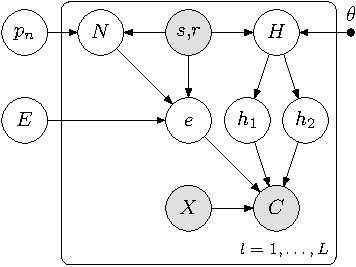
\includegraphics{figures/indelErrorPGMFigureA.pdf}
&
    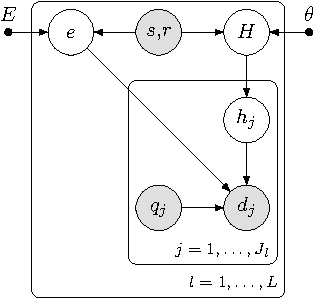
\includegraphics{figures/indelErrorPGMFigureB.pdf} \\
{\bf a} & {\bf b} \\
\end{tabular}
\caption{Structure of the germline indel error and variant calling models in probabilistic graphical model plate notation (some details omitted). {\bf (a) Indel error model.} At each locus $l$, a preliminary estimate of the indel allele count vector $C$ is modeled as a mixture binomial distribution governed by the two true haplotypes $h_1$ and $h_2$ (a function of the unobserved genotype hypothesis $H$), a set of indel error rates $e$ (unobserved) and the total count $X$ (observed). The error rates are selected from the full set of error parameters $E$ according to the sequence context (summarized as an integer pair denoting the size $s$ and number $r$ of STR repeats; observed) and a binary state variable $N$ (unobserved) categorizing the locus as clean (essentially zero error rates) or noisy (prone to indel errors). The genotype $H$ and the noisy-clean state variable $N$ are drawn from prior distributions that depend, respectively, on a context-specific mutation rate $\theta$ shared across samples and a context-specific noisy-state probability $p_n$. {\bf (b) Variant calling model.} The reads $d_j$ at every locus are modeled as depending on the corresponding base call quality strings $q_j$, the unobserved haplotype $h_j$ that generated the read, and the locus-specific error rates $e$. The read-specific haplotype is drawn from the set of haplotypes in the locus-specific hypothesis $H$, of which the prior again depends on a parameter selected from $\theta$ according to context. The error rates are again selected from the global vector $E$ of error parameters (now treated as fixed), with the difference that all loci analyzed by this model are assumed to be in the noisy state.}
\end{figure}

\subsubsection{Indel error count analysis}
At every site that is to be used for the rate estimation process (see Section \ref{sec:error_estimation_implementation}), we need to count the number of reads supporting each potential variant at that site and accumulate these counts by context.

First, the reads are filtered as a pre-processing step based on the following criteria:
    \begin{enumerate}
        \item Read fails platform quality test.
        \item Read is a PCR/optical duplicate.
        \item Read is not mapped.
        \item Read is not a \emph{proper pair}.
        \item Read input alignment contains more than 2 indels.
    \end{enumerate}
Reads with MAPQ scores below 60 are kept but not used to generate the error counts.

The counting process uses a mapped read realignment strategy similar to that used by the variant calling process (section \ref{sec:realignment}), with the following differences:
 \begin{enumerate}
    \item \label{no_threshold_for_indel} There is no threshold for indel candidacy.
    \item \label{no_indel_errors_allowed} No indel errors are allowed when read likelihood for each indel allele is computed.
    \item There is no restriction on the number of overlapping allele candidates based on ploidy.
    \item The whole locus is skipped if more than 4 overlapping allele candidates are found.
    \item The locus is skipped if the set of overlapping alleles at a locus are not all mutually incompatible with the same haplotype. \todo{rephrase, unclear}
    \item Variant and non-variant observations that are within 10 bases of the beginning or end of a read are filtered out.
    \item Error counts are not collected in regions where the pileup depth is more than 3 times the chromosome mean.
 \end{enumerate}

Note that item \ref{no_threshold_for_indel} means that an alignment gap observed once in an input read is treated as a \emph{candidate} for the purpose of error evaluation. Hence, an attempt is made to realign all other reads to that indel, and in the process the likelihood of each read supporting the given indel is found. \todo{do we then pick the maximum likelihood and increment the corresponding hard count?} Item \ref{no_indel_errors_allowed} above means that the read likelihoods are based on explaining the observations via basecalling errors only.

The extracted data are stored in a compact binary file format. A given sequence context $\left\{ s,r \right\}$ has two parameters, short tandem repeat (STR) pattern size ($s$) and STR pattern repeat count ($r$). Each STR tract $i$ with pattern size $s$ and repeat count $r$ at locus $l$ is counted as a single observation for the context $\left\{ s,r \right\}$ and the resulting locus count vector $c_l$ for that observation (with elements $c_l(y), y \in Y,$ corresponding to the observed set of alleles $Y$) is included in the set of locus count observations $C(s,r)$. Reference $N$s are not included. Any ambiguity in the assignment is resolved by choosing the lowest applicable value of $s$ for the site. \todo{perhaps add detail here? Specifically for deciding where the STR begins and ends when there is potential overlap, e.g. is AACAC treated as s=2,r=2 rather than s=1,r=2? How about AAACAC? AAAAAAAACAC? AAAAACACACACACACACAC?}

\subsubsection{Adaptive indel error model parameter estimation}
Every indel locus is modeled as belonging to either a clean state (generating essentially no indel errors) or a noisy state (generating indel errors independently across reads according to a set of error probabilities to be estimated), with the overall error probabilities being drawn from the resulting two-state mixture model. The allele counts, in turn, are modeled as drawn from a mixture over possible genotypes, with the genotype-specific distributions being multinomial for homozygous genotypes and mixtures of two multinomials for heterozygous genotypes. The multinomial distributions are governed by the local coverage  and by rates selected from the vector of available error rates according to the alleles $h_1$ and $h_2$ comprising the genotype (Figure \ref{fig:PGM}a).

Taken together, these model components are a simplified version (based on hard observation counts rather than per-read likelihoods) of the full likelihood model presented later in sections \ref{sec:germline} and \ref{sec:shared}.

For every context $\left\{ s,r \right\}$ we define the following parameters. Together, the $e$ parameters comprise $E(s,r)$:
\begin{itemize}
\item $p_n(s,r)$: the probability of being in the noisy state
\item $e_i(s,r)$: the noisy-state probability of an insertion error resulting in a non-reference variant
\item $e_d(s,r)$: the noisy-state probability of a deletion error resulting in a non-reference variant
\item $e_{\text{ref}}(s,r)$: the noisy-state probability of an indel error resulting in reversion to reference
\item $e_{i,\text{clean}}(s,r)$: the clean-state probability of an insertion error resulting in a non-reference variant
\item $e_{d,\text{clean}}(s,r)$: the clean-state probability of a deletion error resulting in a non-reference variant
\item $e_{\text{ref},\text{clean}}(s,r)$: the clean-state probability of an indel error resulting in reversion to reference
\item $\theta_s(s,r)$: the probability that a locus with the given context has an indel allele.
\end{itemize}
We fix all of the clean-state error probabilities to a small constant value: $1 \times 10^{-8}$. We also set $e_{\text{ref}}$ to $0.01$ during parameter estimation and to a constant factor (1.8) times the corresponding $e_i$ or $e_d$ during variant calling (section \ref{sec:shared})\todo{this parameter is a candidate for adaptive estimation}. The indel mutation rates $\theta_s$ were pre-estimated from chromosomes 1-22 on a fixed training data set and are used as constant values in the current workflow -- this is based on the assumption that the mutation rate does not vary across different sequencing runs or samples. The remaining parameters are estimated on a per-sample basis by maximizing the likelihood of the observed counts:

\begin{equation*}
P(C(s,r) \mid E(s,r), p_n(s,r), \theta(s,r)) = \prod_{l: c_l\in C(s,r)}P(c_l \mid E(s,r), p_n(s,r), \theta(s,r)),
\end{equation*}
where
\begin{equation*}
P(c_l \mid E(s,r), p_n(s,r), \theta(s,r)) = \sum_{H,N} P(N \mid p_n(s,r)) P(H \mid \theta(s,r)) P(c_l \mid N,H,E(s,r)),
\end{equation*}
$H=(h_1, h_2)$ is a variable indicating the specific allele hypotheses under consideration, and $N \in \{ \text{noisy}, \text{clean} \}$ is a variable indicating whether the observation was generated by the noisy or the clean state. For each possible genotype $G \in \{ g_\text{homref}, g_\text{het}, g_\text{homalt}, g_\text{hetalt} \}$ we consider only one hypothesis $H$, obtained by finding the two most likely (by number of supporting counts) non-reference indel alleles $y_1$ and $y_2$ and setting

\begin{equation*}
(h_1, h_2) = \left\{
\begin{array}{lcl}
(\mathrm{ref},\mathrm{ref}) & \mathrm{if} & G=g_\mathrm{het}\\
(y_1,y_1) & \mathrm{if} & G=g_\mathrm{homalt}\\
(\mathrm{ref},y_1) & \mathrm{if} & G=g_\mathrm{hetalt}\\
(y_1,y_2) & \mathrm{if} & G=g_\mathrm{homref}
\end{array} \right.
\end{equation*}

The noisy-state prior is $P(N=\mathrm{noisy} \mid s,r) = p_n(s,r)$; $P(N=\mathrm{clean} \mid s,r) = 1-p_n(s,r)$ and the genotype prior $P(G \mid \theta(s,r))$ is the genomic prior defined in section \ref{sec:germline_genomic_prior}.

For an allele $y$ other than $ref$, $y_1$, and $y_2$, assign the error probability $e(y)$ as $e_i(s,r)$, $e_d(s,r)$, $e_{i,\mathrm{clean}}(s,r)$, or $e_{d,\mathrm{clean}(s,r)}$ according to the value of $N$ and whether $y$ is an insertion or deletion with respect to the reference allele. For $y=\mathrm{ref}$, assign $e(y) = e_\mathrm{ref}(s,r)$ or $e(y)=e_\mathrm{ref, clean}(s,r)$ according to the value of $N$. The probabilities $e(y_1)$ and $e(y_2)$ of errors resulting in $y_1$ and $y_2$ respectively do not need to be assigned specific values due to the approximation below. Finally, let $\bar{e}(h_i)$ be the probability with which $h_i$ is sequenced correctly, with $\bar{e}(\mathrm{ref}) = 1-e_i-e_d$ in the noisy state and $\bar{e}(\mathrm{ref}) = 1-e_{i,\mathrm{clean}}-e_{d,\mathrm{clean}}$ in the clean state.
When  (homref or homalt genotype), the likelihood of the count vector is:

\begin{equation*}
P(c \mid E, n, h_1=h_2) = m_c [\bar{e}(h_1)]^{c(h_1)} \prod_{y \ne h_1} e(y)^{c(y)},
\end{equation*}

where $m_c = \frac{(\sum_{y}{c(y)})!}{\prod_{y}{(c_y!)}}$ is the corresponding multinomial coefficient. Since this coefficient does not depend on any model parameters, it is ignored during parameter estimation.

When $h_1 \ne h_2$ (het or hetalt genotype), the likelihood is:

\begin{equation*}
P(c \mid E, n, h_1 \ne h_2) = m_c [0.5\bar{e}(h_1) + 0.5e(h_1)]^{c(h_1)} [0.5\bar{e}(h_2) + 0.5e(h_2)]^{c(h_2)} \prod_{y \notin \{h_1, h_2 \}} e(y)^{c(y)}.
\end{equation*}

Approximating with $\bar{e}(h_1) + e(h_1) \approx 1$ and $\bar{e}(h_2) + e(h_2) \approx 1$, this simplifies to:
\begin{equation*}
P(c \mid E, n, h_1 \ne h_2) = m_c 0.5^{c(h_1) + c(h_2)} \prod_{y \notin \{h_1, h_2 \}} e(y)^{c(y)}.
\end{equation*}
% Note: fairly high priority to relax the above approximations, particularly when inolving $e_ref$.

Note that this approximation removes the impact of all indel errors that convert between $ref$, $y_1$ and (in the hetalt case) $y_2$. The approximation should lead to a greater distortion of results as indel error rates become large and as greater asymmetry develops between the rate of error from $ref$ to $y_{var}$ vs $y_{var}$ to $ref$.

To reduce the number of estimated parameters, we model homopolymer repeats ($s=1$) with repeat counts $2\leq r \leq 16$ and dinucleotide repeats ($s=2$) with $2\leq r \leq 9$ as log-linear in $r$, allowing us to estimate values for $(s,r) \in \{(1,2), (1,16), (2,2), (2,9)\}$ and interploate between these values. The values at $(1,16)$ and $(2,9)$ are used for $r>16$ and $r>9$ respectively.

When using the estimated parameters for variant calling (Figure \ref{fig:PGM}b, described in section \ref{sec:shared}) we assume that all sites at which candidate haplotypes have been generated belong to the noisy state, so that the mixture model formulation is not needed. For this reason, only the noisy-state error probabilities are passed on for downstream use.
% Note: the main cost of ignoring the clean state may be to reduce recall on homref calls (a metric we care about so little we haven't even bothered to measure it). More generally, it should lower our confidence in calls (whether homref or variants) at clean sites.
We also fix the insertion and deletion error rates to be used for calling to the geometric mean of the insertion and deletion estimates for each STR context.

\subsubsection{Implementation}
\label{sec:error_estimation_implementation}

In practice, the indel error rate estimation is only run on chromosomes which are at least 5 Mb in length. If the combined length of all such chromosomes is less than 50 Mb, indel error estimation is disabled and the method reverts to static parameters for all samples.

If the reference sequence is determined to be acceptable for the estimation process, then the set and ordering of genome regions used to count errors is determined. This is done by finding the subset of chromosomes which are 5 Mb or longer, and dividing each of these chromosomes into the smallest number of approximately equal length segments which are not larger than 2 Mbs each. These intervals are randomly sorted using a fixed seed to help distribute the estimation process over all large chromosomes while providing a deterministic response over multiple runs.

After determining the set and order of estimation intervals, error counting and parameter estimation proceeds independently for each sample. In each sample, counting tasks are launched in order from the estimation interval list up to the number of available workers in the workflow. As each counting procedure completes, the number of sites with non-zero sequence coverage is summed into a running total from all completed tasks. Additional tasks from the estimation interval list are launched until the total coverage of non-empty sites from completed tasks is greater than or equal to 50 Mb. When this site coverage goal is reached, tasks which are no longer needed are canceled, and the workflow waits for tasks to complete so as to cover the smallest continuous series of estimation intervals from the beginning of the estimation interval list which provide coverage of 50 Mb or greater. The workflow waits for this continuous series of tasks so that the final set of counts is deterministic regardless of the completion order of the launched estimation tasks.

Once the counting procedure has completed for a given sample, all of the estimation interval count files are merged, and parameter estimation is conducted according to the procedure outlined above. If parameter estimation fails to converge after the maximum allowed iterations or the estimated error rates fall outside of valid estimation ranges, then the estimation procedure is canceled for the given sample, and the default static parameter set is used for that sample instead.

\subsubsection{Non-adaptive indel error model}
\label{sec:non_adaptive_indel_error}
\todo{I needed to change the equations here to define $e_i$, $e_d$, and $e_{ref}$ as above, am simply guessing that we use $e_i=e_d$ with $e_{ref}$ set the same way as before. Is this correct?}
When adaptive indel error modeling is not enabled, the indel error parameters are set to pre-estimated values based on empirical observation of indel calling performance. The default indel error rates are a function of the homopolymer context length $r$ only; for all other types of indels, including dinucleotide tract indels and mutations of homopolymers which do not represent simple expansion/contraction events, we set $(s,r) = (1,1)$. The indel error rates are set to a log-linear ramp as a function of $r$:

\begin{equation*}
e_i(1,r) = e_d(1,r) = e_{l} \exp(f_r(\log(e_{h})-\log(e_{l})))
\end{equation*}

\noindent where the constant indel errors set for low and high STR lengths are $e_{l} = 5\e{-5}$ and $e_{h} = 3\e{-4}$, and $f_r = \max((r-1),15)/15$.

As a special case, the non-adaptive somatic indel genotyping model uses higher error rates to heuristically account for assembly and mapping errors. This is currently a scaling factor of 100: \todo{Clean up description of this special case.}

\begin{equation*}
e_i(1,r) = e_d(1,r) = 100 * e_{l} \exp(f_r(\log(e_{h})-\log(e_{l}))
\end{equation*}

Finally, $e_{\text{ref}}$ is again set to a constant factor \todo{insert value} times the corresponding $e_i$.


%%%%%%%%%%%%%%%%%%%%%%%%%%%%%%%%%%%%%%%%%%%%%%%%%%%%%%%%%%%%%%%%%%%%%%%%%%%%%%%%%%%%%%%%%%%%%%%%%%%%%%%%%%%%%%%%
%%%%%%%%%%%%%%%%%%%%%%%%%%%%%%%%%%%%%%%%%%%%%%%%%%%%%%%%%%%%%%%%%%%%%%%%%%%%%%%%%%%%%%%%%%%%%%%%%%%%%%%%%%%%%%%%
%%%%%%%%%%%%%%%%%%%%%%%%%%%%%%%%%%%%%%%%%%%%%%%%%%%%%%%%%%%%%%%%%%%%%%%%%%%%%%%%%%%%%%%%%%%%%%%%%%%%%%%%%%%%%%%%
\section{Variant calling workflow}

Following all preliminary parameter estimation tasks, the primary variant calling operation is initiated. Variant calling tasks can be divided among a set of worker processes running in parallel, with each worker process handling one or more segments of the genome. For each genome segment, a worker process completes all phases of variant calling described below in a single operation transitioning from the lowest to highest position in the targeted genome segment. When all genome segments have been processed their intermediate results are merged into the complete output files.

\paragraph{Genome segmentation} Given a maximum segment size (default is 12 Mb), each chromosome is partitioned into a set of nearly equal size segments such that each does not exceed the maximum. Each genome segment larger than 200Kb can be directly distributed to a worker process for variant calling, smaller segments are grouped together such that each worker process handles a batch of genome segments which have a total length of less than 200Kb. Grouping small segments better amortizes the startup and bookkeeping costs of each variant calling process in cases where large numbers of small contigs need to be handled, such as for decoys and unplaced contigs in the human hg38 reference.

\paragraph{Segment boundaries} When a chromosome is divided into multiple segments, it is important that variant calling results across segment boundaries are identical to the results of calling the entire chromosome using a single variant calling process. To ensure that this is the case, in each variant calling process the targeted genome segment is expanded by a fixed size to create small border regions preceding and following the original target region. In these border regions the variant caller completes all parts of the variant calling operation except for writing any output. In this way regional operations such as haplotype modeling will be applied consistently across segment boundaries. The region expansion size is 100 bases plus the variant caller's maximum indel size (50). In the case of germline calling, the expansion size is further increased by the haplotype model's maximum active region size (250).


%%%%%%%%%%%%%%%%%%%%%%%%%%%%%%%%%%%%%%%%%%%%%%%%%%%%%%%%%%%%%%%%%%%%%%%%%%%%%%%%%%%%%%%%%%%%%%%%%%%%%%%%%%%%%%%%
%%%%%%%%%%%%%%%%%%%%%%%%%%%%%%%%%%%%%%%%%%%%%%%%%%%%%%%%%%%%%%%%%%%%%%%%%%%%%%%%%%%%%%%%%%%%%%%%%%%%%%%%%%%%%%%%
%%%%%%%%%%%%%%%%%%%%%%%%%%%%%%%%%%%%%%%%%%%%%%%%%%%%%%%%%%%%%%%%%%%%%%%%%%%%%%%%%%%%%%%%%%%%%%%%%%%%%%%%%%%%%%%%
\section{Variant discovery and evidence filtration}

%%%%%%%%%%%%%%%%%%%%%%%%%%%%%%%%%%%%%%%%%%%%%%%%%%%%%%%%%%%%%%%%%%%%%%%%%%%%%%%%%%%%%%%%%%%%%%%%%%%%%%%%%%%%%%%%
\subsection{Input read processing}

The input alignment files are scanned for reads as the first step of the variant calling operation. Reads are immediately filtered out if they are marked as not passing primary analysis filters, PCR/optical duplicates, unmapped, secondary or supplemental. The remaining reads are categorized to determine how the read will be used in downstream steps. The categories are
\begin{enumerate}
    \item Tier1 reads have the most reliable alignments. These are used for all aspects of variant calling.
    \item Tier2 reads have less reliable alignments than tier1. These are used for verification of somatic calls as described further below.
    \item Sub-mapped reads have the least reliable alignments. These are retained, together with tier1 and tier2 reads, to enable  variant classification features, such as the root mean square mapping quality for all reads covering a variant locus.
\end{enumerate}

For the germline and somatic calling models reads are classified as tier1 if they have a mapping quality of 20 or higher, and if paired, a mate read which is mapped and marked as a \emph{proper-pair}. All other unfiltered input reads are classified as sub-mapped in the germline model and as tier2 reads in the somatic model.

Input read alignments are also normalized as follows:
\begin{enumerate}
    \item Indels are left-shifted (moved to a lower position) such that the total number of alignment mismatches does not increase with each single-base left-shift operation.
    \item Adjacent indels are merged, for instance the alignment indicated by CIGAR `10M1I2I10M' would be simplified to `10M3I10M' and `10M2D1I3D10M' would be simplified to `10M5D1I10M'
    \item Indels are simplified by identifying any portion of a set of adjacent insert/delete edits which can be matched to the reference, for example, given reference `ACTGC' and read `ACGC', the CIGAR `2M1I2D1M' will be simplified to `2M1D2M'
    \item Indels on (or left-shifted to) the edge of the read are simplified, possibly changing the alignment start position. For instance an alignment CIGAR of `1D10M' at position 100 is transformed to `10M' at position 101.
\end{enumerate}
These normalization steps do not alter the alignment's soft-clipping.

%%%%%%%%%%%%%%%%%%%%%%%%%%%%%%%%%%%%%%%%%%%%%%%%%%%%%%%%%%%%%%%%%%%%%%%%%%%%%%%%%%%%%%%%%%%%%%%%%%%%%%%%%%%%%%%%
\subsection{Haplotype model}

Each sample's ploidy introduces constraints that can be used to reduce errors due to sequencing noise, incorrect read mapping, inconsistent alignment to low-complexity sequence and regions where the reference serves as a poor template for the sample. In a simple haplotype model, such as that described in FreeBayes \cite{garrison2012}, candidate haplotypes can be identified from existing read alignments. More advanced haplotype generation methods are less dependent on the input read alignments, often using local assembly as a means to identify longer consensus haplotypes in the context of sequencing noise and high levels of variation from the reference, such as the haplotype generation methods used in Platypus \cite{rimmer2014} and GATK HaplotypeCaller \cite{depristo2011}, among others.

Strelka's germline caller uses a haplotype modeling step combining both simple alignment-based and assembly-based approaches to haplotype generation, where the appropriate method is selected for each region to optimize runtime without loss of calling precision. Candidate haplotypes are processed through various denoising steps and regional complexity statistics are made available to the variant caller's end-stage empirical variant scoring scheme to reflect reduced variant-calling confidence in regions where sequencing data poorly fit the expected haplotype count. Note that no haplotype modeling is currently attempted during somatic variant calling.

The full haplotyping procedure is comprised of the following steps: (1) detecting short clusters of sequence variation called {\em active regions}, (2) generating candidate haplotypes in active regions, (3) filtering candidate haplotypes to reduce noise, and (4) decomposing the remaining candidate haplotypes into primitive alleles such as SNVs and short indels. The haplotype modeling procedure is currently run independently for each sample. For runtime efficiency, active regions are constrained to be $\leq 250$ bases by default.


\subsubsection{Active region detection}
To detect active regions, we first identify loci that are likely to have variants, which we call {\em variant loci}. To identify variant loci, for each locus we calculate an alignment depth (the number of alignments overlapping the locus) and a variant evidence count (weighted count of alignments with variants at the locus). Variant evidence counts are updated while reading alignments. A mismatch of an alignment at locus $i$ increases the counter at locus $i$ by 1. An insertion of a sequence between locus $i$ and $i+1$ increases the counters at $i$ and $i+1$ by 4. A deletion of loci $[i,j]$ increases the counters in $[i-1,j]$ by 4. Similar to an indel, a soft-clipped segment ending (starting) at locus $i$ increases the counter at $i$ and $i+1$ ($i-1$) by 4. After all alignments overlapping a locus are read, a decision is made whether the locus is a variant locus. A locus with a variant evidence count $c$ and an alignment depth $d$ becomes a variant locus if (1) $c \geq 0.35 \cdot d$ or (2) $c \geq 9$ and $c \geq 0.2 \cdot d$.

After variant loci have been detected, nearby variant loci are clustered if they are within 13 bases of each other. For the clusters including two or more variant loci, the cluster region is further extended to the surrounding loci so that the first and last locus are not within a homopolymer or short tandem repeat (STR) region. This extension is needed because alignments that do not fully span such repeats are often erroneous and relying on them may lead to generating incorrect haplotypes. To accomplish this, we detect {\em anchor loci} that are not variant loci and also do not belong to a homopolymer (of lengths no less than 3) or STR (of repeat unit lengths between 2 and 50). Given a cluster of variant loci, the active region is created between the closest anchor loci before and after the first and last variant loci.

Note that the active region detection method is designed so that the vast majority of indels are included in active regions. Even for a single base deletion at locus $i$, each alignment having the deletion increases the counters at $i-1$ and $i$ by 4, thus only three of such alignments trigger creation of an active region including $i-1$ and $i$.


\subsubsection{Haplotype generation}
Given an active region of size of 250 or smaller, haplotype generation is attempted using either simple counting or local de novo assembly. The simple counting method relies on the majority of supporting reads spanning the entire active region. It is appropriate to quickly generate haplotype candidates for relatively short active regions with simple variation or noise patterns. Local assembly of the locus is more costly but better able to resolve complex variation and interactions with STRs. The decision to run counting or assembly is based on the fraction of reads that fully cover the active region (called covering reads). Simple counting is used for haplotype generation, unless fewer than 65\% of all reads that overlap with an active region are covering reads, in which case local assembly is used.

If simple counting is selected, then for each covering read, the segment aligned to the active region is extracted as a candidate haplotype. If a candidate haplotype $s$ is extracted from a read $r$, we call $r$ a supporting read of $s$, such that for each candidate haplotype $s$ a set of supporting reads is identified.

If assembly is selected, local de novo assembly is run using a de-Bruijn graph approach (detailed in \ref{sec:HaplotypeAssembler}). Prior to assembly the target active region is expanded to avoid having the active region start or end within an STR as a means to improve the identification of contigs which span the full locus. Active region expansion occurs as follows: given an active region $[i,j]$, we extend it up to 9 bases upstream and downstream until it encounters a variant locus. Thus the expanded active region $[i',j']$ satisfies the following conditions: $i-9 \leq i' \leq i$, $j \leq j' \leq j+9$, and there is no variant locus in $i' \leq pos \leq i-1$ and $j+1 \leq pos \leq j'$. Since $i$ and $j$ are anchor loci, this extension allows the identification of assembled contigs which span the full locus by identifying those that share the same prefix (reference segment at $[i',i]$; denoted by a prefix anchor) and suffix (reference segment at $[j,j']$; denoted by a suffix anchor). All the reads that (fully or partially) overlap with the expanded active region are used as input to the assembly procedure. For the sake of speed, if the number of reads exceeds 1000, assembly is not performed. After assembly is finished, from all the contigs returned by the assembler, only the contigs including both prefix and suffix anchors are selected. After removing the prefix and suffix anchors, each such contig becomes a candidate haplotype $s$, and the set of reads supporting the contig is identified.

Haplotype generation for an active region is considered unsuccessful if the assembly procedure is selected and assembly is unable to generate at least one non-reference candidate haplotype. If haplotype generation does not succeed, indel candidates can still be generated without the benefit of a local haplotype hypothesis as described in \ref{sec:IndelCandidacy}.

\subsubsection{Haplotype assembly}
\label{sec:HaplotypeAssembler}

Given an expanded active region, all reads (fully or partially) aligned to the region are gathered, and for each such read, the segment aligned to the region is extracted and used as an input to assembly. If the overlapping portion of the read includes a soft-clipped segment, the entire soft-clipped segment is extracted. If the length of the extracted read segment is less than the sum of prefix and suffix anchor lengths, they are filtered out. The selected read segments are assembled using a simple algorithm implicitly based on the popular de Bruijn graph approach originated by Pevzner \textit{et al}. \citep{pevzner2001}. We note here that the orientation of each unmapped assembly read is determined by the orientation of its mapped partner, avoiding the need to deduce this during the assembly. Assembly is attempted over a series of word sizes, starting from a minimum value which is increased until repeat filtration criteria are met or the maximum word size is reached. The method currently uses the sum of prefix and suffix anchor lengths as the minimum word size and 76 as the maximum word size, the word size is incremented by 3.

For a given word size $k$, a word list is made of all $k$-mers present in the input reads. A seed list, as a subset of the word list, is also made by excluding the circular $k$-mers that form any cycle in the graph. The most frequent $k$-mer in the seed list, given it has the most supporting reads, is selected as a seed for the resulting contig assembly. The contig is extended from that seed in each direction by choosing $k$-mers from the word list having a $k-1$ overlap with the contig end. To avoid haplotype switching, reads that support the contig are tracked at each extension point. When there are multiple potential extensions, a $k$-mer is selected so that the current extension has the highest consistency of supporting reads with the previous extensions. The extension ends when there is no overlapping $k$-mer from a previous supporting read, or when the selected $k$-mer is circular. The contig is then collected, and each $k$-mer used to construct the contig is removed from the seed list if contained. The contig construction procedure is repeated to generate multiple contigs until all seeds in the list are exhausted. If any of the returned contigs ends at a circular $k$-mer, the word size is incremented by one step, and the contig assembly procedure is restarted. All the contigs generated with the previous word size are treated as pseudo reads which are input into the next assembly iteration, similar to the utilization of pseudo reads described in \cite{tigra2014}.

Finally, a greedy procedure is applied to select the constructed contigs in the order of the number of effective supporting reads and contig length. An effective supporting read cannot be a pseudo read, nor support any contigs that have been selected previously. The selection process is repeated until either there are no more contigs available with the minimum number of effective supporting reads (defaults to 2), or the maximum number of contigs are assembled (defaults to 10).

\subsubsection{Haplotype filtration}

If haplotype generation is successful (using either counting or assembly methods), then haplotype candidates are next filtered to reduce potential noise.

The first noise reduction step identifies and filters candidates based on the expected sample ploidy (assumed to be diploid in the current procedure). To do so, the candidate haplotypes are ranked by decreasing number of supporting reads after removing any candidates with less than 3 supporting reads. Among the set of candidates with the highest level of read count support, the first one generated in the candidacy process is selected and removed from the ranked list. The set of candidates with the highest number of supporting reads in the remainder of ranked list are also selected, but only if this would result in a total of 2 or fewer non-reference selected haplotypes. Any non-selected candidate haplotypes are filtered from further consideration.

If there is more than one remaining haplotype, an additional filtration step is applied to reduce candidates produced by phasing noise in the sequencing process across a homopolymer. The test assumes that the candidate haplotype with the highest read support, $h_1$ is true, and identifies whether the candidate haplotype with next highest level of read support, $h_2$ is a phasing noise artifact introduced while reading $h_1$. The conditions which trigger this filter are as follows (1) $h_1$ and $h_2$ are the same length with only one mismatching basecall (2) all reads supporting $h_2$ are observed on only one strand and (3) the basecall mismatch between $h_1$ and $h_2$ occurs at one of the ends of the sequence, and causes $h_2$ to contain an uninterrupted homopolymer at least 11 bases long. If these conditions are met, all haplotype candidates besides $h_1$ are filtered from further consideration.

\subsubsection{Primitive allele discovery}
After filtration, the remaining candidate haplotypes are aligned to the reference using a global aligner that employs an affine gap penalty function with the following parameters: match score 1, mismatch penalty 4, gap opening penalty 5, and gap extension penalty 1. From the alignment, primitive alleles (SNVs and indels of size 50 and smaller) are identified and marked {\em discovered} in an active region. These discovered primitive alleles are used to improve SNV and indel calling by (1) relaxing the mismatch density filter (described in \ref{sec:MismatchDensityFilter}), (2) improving indel candidacy (described in \ref{sec:IndelCandidacy}), and (3) phasing SNVs and indels within the same active region (described in \ref{sec:ReadBackedPhasing}).

%%%%%%%%%%%%%%%%%%%%%%%%%%%%%%%%%%%%%%%%%%%%%%%%%%%%%%%%%%%%%%%%%%%%%%%%%%%%%%%%%%%%%%%%%%%%%%%%%%%%%%%%%%%%%%%%
\subsection{Indel candidacy}
\label{sec:IndelCandidacy}

Strelka uses indel candidacy as a preliminary filter to eliminate indel observations from consideration as variants if they are very likely to have been generated by error processes. Any indel which becomes a candidate will be considered during read realignment and indel genotyping in all samples.

To become a candidate, an indel variant must minimally have 2 reads supporting it in at least one sample. If haplotype modeling is enabled, a candidate indel belonging to an active region where haplotyping was successful must also have been discovered through haplotype alignment in at least one sample. If an indel observation satisfies these conditions, Strelka evaluates its candidacy status using a one-sided binomial exact test, with the null hypothesis being that the indel coverage is generated by indel error processes.

Given a total locus coverage of $N$, indel coverage of $n_i$, and an indel error rate of $e_l$ \todo{the rest of this document is written so as to support separate insertion and deletion rates (even though currently equal to each other) - make this description compatible with that}, we define the probability of some coverage $x$ being generated at the locus due to indel error as
\begin{equation*}
P(x \mid N, e_l) = \binom {N} {x} e^{x}_l (1 - e_l)^{N - x}
\end{equation*}
We can then define the probability of generating an indel with at least coverage $n_i$ due to indel error at a locus as follows:
\begin{equation*}
p_{error} = P(X >= n_i \mid N, e_l) = \sum_{x = n_i}^{N} P(x \mid N, e_l)
\end{equation*}

\noindent The indel is considered a candidate variant if $p_{error} < p_{reject}$, where $p_{reject}$ is the rejection threshold for the null hypothesis. The default value of $p_{reject}$ is $1\e{-9}$.

\paragraph{External candidate input}

The above process describes how indel candidates are discovered from the input read alignment either directly or via additional processing in the haplotype model. Strelka also allows the user to specify indel candidates from one or more VCF files. Each such indel VCF can optionally include a \emph{forced genotype} specification, which means that the given indel allele must be genotyped and emitted in the VCF output, even when there is no evidence to support the allele. Regardless of the \emph{forced genotype} status, all external candidates input are automatically considered candidate variants and are treated in subsequent realignment and genotyping stages in the same way as a candidate discovered directly from the input alignment data.

\ifx\IncludeDevelopmentDetail

\paragraph{Design discussion}

The current indel candidacy test is suspected to be a poor fit to indel error behavior in the data. This particular combination of model, input parameters and rejection thresholds empirically functions reasonably well, but there is poor theoretical justification for all three. It would be particularly beneficial to revamp this model to be compatible with adaptive indel estimation in future work.


\begin{raggedParagraph}{Implementation details}

The indel candidacy test is contained in class \verb|IndelBuffer|, and triggered by its predicate method \verb|isCandidateIndel|. The above described candidacy logic is primarily implemented in \verb|isCandidateIndelImplTest|. To achieve a practical runtime the above described binomial p-value test is implemented using a cached Poisson approximation to the binomial, as implemented by helper class \verb|min_count_binom_gte_cache|.

\end{raggedParagraph}

\fi % IncludeDevelopmentDetail


%%%%%%%%%%%%%%%%%%%%%%%%%%%%%%%%%%%%%%%%%%%%%%%%%%%%%%%%%%%%%%%%%%%%%%%%%%%%%%%%%%%%%%%%%%%%%%%%%%%%%%%%%%%%%%%%
\subsection{Read realignment}
\label{sec:realignment}

Following the discovery of candidate alleles (optionally including haplotype modeling), reads are realigned in the context of these candidates. This realignment step has two primary functions. The first is to generate the set most likely alignment for the read when constrained to various alternate alleles at each locus. Such alignments are used to assess the read's relative support for different indel alleles as part of downstream indel calling models (more detail on this usage is described in \ref{sec:PerReadLikelihood}). The second function is to create a single \textit{representative} alignment to use for SNV calling, as detailed further below.

\subsubsection{Alignment search}
The alignment search used during the realignment step assumes at least one gapless block of each starting alignment is already correct, and thus can be used to seed an improved alignment based on a sparse set of intersecting candidate indels. The search proceeds as follows. Each read has a starting alignment provided by some input alignment file, as well as a trial indel set. This trial indel set contains intersecting candidate indels, in addition to any non-candidate indels already present in the starting alignment. If the read does not intersect any candidate indels, no realignment is performed, and the search procedure returns only the input read's starting alignment.

If the read does intersect at least one candidate indel, a set of alignments is built from the starting alignment by recursively toggling indels from the trial set. Each such indel toggling operation will produce three alignments derived from the input alignment. One of these is the input alignment itself, representing the trivial case of not toggling the indel. The other two alignments are found by adding or removing the indel in question such that the input alignment is unchanged (1) to the left of the indel or (2) to the right of the indel. For example, consider an input alignment at position 10 with an alignment of \texttt{100M}, and a trial indel set consisting of one indel, a 1 base deletion at position 50. In this case the search procedure will produce three candidate alignments: (1) position 10 with alignment \texttt{100M} (2) position 10 with alignment \texttt{40M1D60M}, and (3) position 9 with alignment \texttt{41M1D59M}.

As the above procedure recursively executes on each indel in the trial set, new candidate indels are added to the trial set when intersected by a derived alignment extending beyond the range of its source. Note that for RNA input, the above procedure will be executed independently for each exon.

This search process is efficient for the case where a read intersects only one or two candidate indels. Due to the complexity being exponential in trial set size, heuristics are used to curtail the alignment search in regions with high candidate indel density. Specifically, the search recursion depth is limited to no more than 5, and will be set lower if required such that the number of enumerated alignments does not exceed 5000.

\subsubsection{Soft-clipped segment handling}

By default, prior to a read being realigned, any soft-clipped segment on the leading and trailing edge of the starting alignment is unrolled to force the segment to be aligned to the reference. This treatment assumes that most soft-clipping reflects an indel which has not yet been included in the read's starting alignment.

\subsubsection{Creation of a representative alignment}

The representative read alignment used for SNV calling is usually the most probable alignment, but some allowance is made for an alignment which is nearly the most likely yet more parsimonious. To do so, the likelihood of each alignment is found (as described in section \ref{sec:PerReadLikelihood}), and any alignment with a likelihood within a factor of 10 of the most likely is entered into a pool of alignment candidates which are eligible to be chosen as representative. Within this eligible pool of alignment candidates, the representative alignment is chosen if it has the (1) fewest indels, (2) fewest non-candidate indels, (3) lowest total insertion length, or (4) lowest total deletion length. The criteria are applied in the order given and the first to produce a representative is used.

If the eligible pool of alignment candidates has more than one member, additional soft-clipping may be added on the edges of the representative alignment such that any conflicting alignments on the edge of the read within the eligible alignment pool are removed. This soft-clipping step is helpful for cases such as an alignment which partially covers an STR, causing alignments to the reference and indel alleles to be equally likely. In such an instance the portion of the alignment extending into the STR is soft-clipped.

For RNA analysis the above procedure is slightly adjusted. First, the eligible pool of representative alignment candidates is pruned to only consider those which preserve exon-intron boundaries provided in the starting alignment. Second, the procedure described above to 'unroll' soft-clipped segments from the starting alignment is still used for RNA analysis, but an additional check is made to see if the starting alignment is more likely than any alternative proposed by the alignment search process. If this is the case, the starting alignment is used as the representative alignment instead.

\ifx\IncludeDevelopmentDetail

\paragraph{Design discussion}

The unconventional alignment search method used here has favorable runtime when its input assumptions are approximately true; however, this comes with several costs. (1) The complexity of the search method is exponential in the number of indels intersecting the alignment. As discussed above, this is mitigated with heuristics but remains a problematic feature. (2) It assumes that the likelihood of a read for a given haplotype will be approximated by a single most likely alignment. A pairHMM could improve on this approximation with a more precise approach. (3) The method introduces substantial additional code complexity.

\begin{raggedParagraph}{Implementation details}

Read realignment is executed once for each read, starting from the entry-point function \verb|realignAndScoreRead|, from which all alignments are enumerated for the read in the private function \verb|getCandidateAlignments|. Representative alignment selection and soft-clipping is implemented by the function \verb|scoreCandidateAlignments|.

\end{raggedParagraph}

\fi % IncludeDevelopmentDetail

%%%%%%%%%%%%%%%%%%%%%%%%%%%%%%%%%%%%%%%%%%%%%%%%%%%%%%%%%%%%%%%%%%%%%%%%%%%%%%%%%%%%%%%%%%%%%%%%%%%%%%%%%%%%%%%%
\subsection{Basecall quality adjustment and filtration}

\subsubsection{Mapping error adjustment}

For both germline and somatic SNV models, basecall error probabilities are adjusted to reflect the joint probability of sequencing and read mapping error. The adjusted basecall error probability is

\begin{equation*}
e_{b^{\prime}} = (1-e_m)e_b + e_m 3/4
\end{equation*}

where $e_b$ is the basecall error probability estimated by the sequencer and $e_m$ is the read mapping error probability.


\subsubsection{Basecall filtration}
\label{sec:BasecallFiltration}
Following read realignment and mapping error adjustment, additional basecall filtration steps are conducted for SNV calling and depth estimation. This filtration has two intended purposes, (1) to filter noisy obsevations from the SNV calling process, and (2) to provide statistics on the fraction of basecalls filtered at each site. The filtered basecall fraction may be used in downstream variant filtration routines (see section \ref{sec:FiltrationAndScoring}). Note that these steps do not impact indel calling.

The first filtration stage consists of a single step to trim off any contiguous series of ambiguous basecalls from the end from the read. Any basecalls trimmed off in this stage are not recorded in the counts of filtered basecalls at each site used for downstream variant filtration.

The steps of the second filtration stage are:

\begin{enumerate}
    \item In the germline SNV model, basecalls with mapping-adjusted qualities of 17 or less are filtered out. No such filtration is used by the somatic SNV model.
    \item Any ambiguous basecalls remainng after the first filtration stage are filtered out.
    \item The \textit{mismatch density filter} (described below) is applied to a basecall if the local read context is highly diverged from the reference or a local haplotype candidate.
\end{enumerate}

Any basecalls trimmed off in the second stage are  recorded in the counts of filtered basecalls at each site, and thus may impact downstream variant filtration.

\paragraph{Mismatch density filter}
\label{sec:MismatchDensityFilter}

The mismatch density filter is run on all reads to mask out sections of the read having an unexpectedly high density of disagreements with the reference or other locally proposed haplotype candidates. This filter removes a basecall from consideration if more than $M$ mismatches occur between the read and the reference within a window of 41 bases. This 41 base window is typically centered at the site in question unless restricted by the edge of the read, in which case it extends 41 bases into the read from the edge. Note that each indel is counted as as a single mismatch, and that differences with the reference that agree with a local haplotype candidate are not counted as mismatches for the purpose of this filter (see below).

For germline variant calling, the mismatch threshold $M$ is set to 2. For somatic variant calling $M$ is set to 3 when calling at the tier1 evidence level and 10 at the tier2 level (see section \ref{sec:SomaticEvidenceTiers}).

The haplotype model used during germline calling enables this filter to be applied more precisely by ignoring mismatches corresponding to local candidate haplotypes. To improve the degree to which this filtration is consistent across of set of jointly analyzed samples, an SNV from a candidate haplotype proposed in any sample can be used in all samples to prevent counting the corresponding base as a mismatch for filtration purposes.


\ifx\IncludeDevelopmentDetail

\paragraph{Design discussion}

Given a haplotype model applied to all calling modes (including somatic), we could eliminate the mismatch density filter and instead apply a term expressing 'how surprising is this haplotype given level X of divergence from the reference?' as part of the genotype stage. On the other hand, if there is a long-term need for such a filter, it would be helpful to eliminate the fixed window size of 41, and instead weigh mismatches as a function of distance from the call position.

\begin{raggedParagraph}{Implementation details}

Most basecall filtration steps are executed in method \verb|starling_pos_processor_base::pileup_read_segment|. The mismatch density filter in particular is efficiently precomputed for each read in the \verb|create_mismatch_filter_map| function.

\end{raggedParagraph}

\fi % IncludeDevelopmentDetail

%%%%%%%%%%%%%%%%%%%%%%%%%%%%%%%%%%%%%%%%%%%%%%%%%%%%%%%%%%%%%%%%%%%%%%%%%%%%%%%%%%%%%%%%%%%%%%%%%%%%%%%%%%%%%%%%
\subsection{Overlapping indel filtration}

Following candidate allele identification and realignment, additional steps are taken in both the germline and somatic variant calling pipelines to filter excessive numbers of overlapping/conflicting candidate alleles at the same locus. In the germline model this filtration is based on the ploidy of the region and serves a similar role to the filtration performed in the earlier haplotype modeling step. In the somatic model this filtration is performed without any attempt to estimate the characteristics and number of tumor sub-clones, so it is currently employed as an heuristic approximation.

\subsubsection{Overlapping indel filtration in the germline caller}
In the germline model, indel filtration is based on the expected ploidy $p_s$ that is specified by region for each sample $s$. Ploidy values of $1$ and $2$ are currently supported, with a default value of $2$ if not specified as input to Strelka. We restrict the downstream analysis to consider only the $p_s$ most likely alleles, plus the reference allele if it is not already contained in the list.

As mentioned above, this process partially replicates the ploidy-based noise filtration that occurs in the haplotype model, but it remains an important step because (1) there are variant loci where the haplotype model does not operate for various reasons, for instance because no active region was triggered, assembly failed, the region was too large, etc., and (2) the overlapping allele filtration step described below is different than that performed in the haplotype model in that it occurs after read realignment and is based on the likelihood of reads to support each of the overlapping alleles in question, rather than being based on simple read counts.

The position of an indel is assigned as the first position following the left-most breakpoint of the left-shifted indel. This means that overlapping alleles need not share the same position, and that the list of indel candidates considered at a given position may also need to contain alleles at other nearby positions. For each sample, the filtered list of candidate indels is constructed in two stages. First, we identify all indel alleles at the position of interest, rank them by read likelihood support, and retain the $p_s$ (or $p_s+1$) highest-ranking alleles. All alleles in this list necessarily overlap with each other. Second, we expand the list by adding indel alleles at other positions, subject to the condition that all of the alleles in the final list must again overlap with each other. We again rank this list by read support and retain the top $p_s$ (or $p_s+1$) alleles. These two steps are described in more detail below.

\paragraph{Constructing a list of overlapping indels indexed to a single position}

Each position in the genome is processed in left to right order. For each position, the first step in indel calling is to find the set $A$ of all indel candidate alleles at that position in addition to the reference allele. For each sample $s$, all reads in that sample $d \in D_s$ are identified for which the read likelihood $P(d \mid a)$ has been computed for all alleles $a \in A$ \todo{link to the criteria used to decide whether to compute $P(d \mid a)$, this should be something like "the read overlaps a breakpoint of $a$  by at least 5 bases, and the likelihood for the reference allele is always included"}. Note the set of reads found for this purpose is not restricted to tier1 reads. The allele likelihood for each read $P(d \mid a)$ is transformed to an allele probability $P(a \mid d)$ assuming a uniform prior on $A$, such that the total support $t_s(a)$ for each allele $a$ in the sample can be found from

\begin{equation}
\label{eq:perSampleAlleleSupport}
t_s(a) = \sum_{d \in D_s}{P(a \mid d)}.
\end{equation}

Within each sample, alleles are assigned a rank $k_s(a)$ from highest to lowest $t_s(a)$ values. The top-ranked $p_s$ alleles are selected for consideration in the next processing step. If the reference allele was not in the top $p_s$ alleles, it is added into the set as well. This process yields the filtered allele set $A^{\prime}$.
\begin{comment}
% Commenting out for now because forced genotype indel writeup is being deprioritized until other sections are done.
Note that any \emph{forced genotype} indel alleles removed from consideration here will be revisited in a subsequent step to ensure that they are genotyped and emitted in the final VCF output.
\end{comment}

\paragraph{Extending the list to consider indels indexed to other positions}

The next step of the locus allele-selection procedure resolves any additional overlapping indels at other positions, if these exist. To do so, we first define \emph{overlapping indels} as two indels which intersect or are adjacent, such that they could not both be present in the same haplotype. In the procedure below we are constrained to only consider a set of alleles for filtration (and subsequently genotyping), where all alleles in the set are overlapping.

All indels indexed to locations other than the targeted position which overlap all alleles in $A^{\prime}$ are found, forming the extended candidate allele set $A_x$. As above, the total read support for each of these alleles is used to generate a per-sample ranking of the extended allele set $k_s(a), a \in A_x$. This per-sample rank is used to generate a heuristic sum of ranks over all samples which provides an approximate score for ranking alleles across all samples

\begin{equation*}
t(a) = \sum_{s \in S}{\setSize{A_x} - k_s(a) + 1}
\end{equation*}

$B$, a mutually-overlapping superset of $A^{\prime}$, is then found using the following iterative procedure. $B$ is initialized to contain all alleles in $A^{\prime}$, Each allele $a \in A_x$ is tested in order from highest to lowest $t(a)$ value, to see if it overlaps with all alleles in $B$. If so, the allele is added to $B$, before iterating to the next lowest-scoring allele in $A_x$.

As a final step, per-sample allele support is computed for the combined extended allele set $B$, as in equation \ref{eq:perSampleAlleleSupport} above, to find the per-sample allele support $t_s(a), a \in B$. This support is then used to rank alleles in each sample and apply ploidy-based filtration for each sample to produce the final set of alleles to be evaluated at each locus.


\begin{comment}
% Commenting out for now because it is not clear where the global ranking has any important impact on inference. It does impact the order the alleles are written to the VCF record, but does it do anything more substantial?

Global allele Ranking

Following the ranking and selection of top alleles in individual samples, alleles are ranked over based on a sample-wide support score $t(a)$. This is found by a simple heuristic based on the sum of per-sample ranks computed above

\begin{equation*}
t(a) = \sum_{s \in S}{\max(0, p_s - k_s(a) + 1)}
\end{equation*}

\end{comment}


\begin{comment}

\paragraph{Recovering forced genotype indels}
% Commenting out for now because forced genotype indel writeup is being deprioritized until other sections are done.

Indels which have been marked with a \emph{forced genotype} status must be genotyped and emited in the output VCF even if there is no supporting evidence for them in the sample. The purpose of this output is to allow the absence of the allele to be asserted in a way that can be distinguished from low-coverage or inability of the sequencing reads to differentiate thee allele (due to, e.g. a long STR). Any forced genotype indels which have been filtered from the standard genotyping process by the above processes are re-evaluated individually in a separate pipeline to genotype and emit forced indels which are not output as variants.

IT works like this....

\end{comment}


\ifx\IncludeDevelopmentDetail

\paragraph{Design discussion}

The above procedure should be improved on at least two primary directions. (1) It acts almost independently of the haplotype model, while fulfilling a similar role (ploidy-based noise filtration), so it should be adapted to act at the haplotype level when this information is available, while retaining an ability to function on those loci where haplotype assembly may occasionally not succeed. (2) It should more consistently treat SNVs, so that it simply becomes overlapping \emph{allele} resolution, instead of a step specific to indels.

In a similar direction to haplotye model incorporation, the definition of overlapping alleles used here is limiting, in that the indels are only considered in their left-shifted positions. Ideally the above procedure would move to whole haplotype ranking and selection, but where evaluation of individual alleles is required, these should be considered as sequence replacements over the entire STR tract they impact.

As noted in the methods above, allele ranking and noise filtration does not employ any population genetics model and is not expected to perform well in large cohorts. For the targeted use case of individuals and small families it is observed to perform well.

\begin{raggedParagraph}{Implementation details}

    The entry point for these procedures are in method \verb|starling_pos_processor::process_pos_indel_digt()|.

\end{raggedParagraph}

\fi % IncludeDevelopmentDetail


\subsubsection{Overlapping indel filtration in the somatic caller}

The somatic model uses some similar approaches as the germline model for overlapping candidate indel filtration. In the somatic model's approach, each candidate indel allele is evaluated as an independent operation. For the candidate indel in question, all overlapping candidate indels (at any starting position) are found, and together with the reference allele form the overlapping indel allele set $A$. Next, all reads in both the tumor and normal samples $d \in D$ are identified for which the read likelihood has been computed for alleles $a \in A$ \todo{link to the criteria used to decide to compute the read likelihood}. The allele likelihood for each read $P(d \mid a)$ is transformed to an allele probability $P(a \mid d)$ assuming a uniform prior on $A$, such that the total support $t(a)$ for each allele $a$ can be found from

\begin{equation*}
\label{eq:perSomaticModelAlleleSupport}
t(a) = \sum_{d \in D}{P(a \mid d)}
\end{equation*}

The candidate indel in question is filtered from consideration in the somatic variant calling pipeline if its support score $t(a)$ is not in the top 2 among all $a \in A$. Additionally, the candidate indel is filtered out if a 3rd allele exists and it has greater than 10\% support among the top 3 alleles.

\ifx\IncludeDevelopmentDetail

\paragraph{Design discussion}

This filter is likely to be too broad, possibly removing large numbers of TP for a small gain in precision. It should be replaced with a haplotype model adapted for the somatic case.

\begin{raggedParagraph}{Implementation details}

The filtration test is implemented in the predicate \verb|is_multi_indel_allele|, as part of the \verb|somatic_indel_grid.cpp| module.

\end{raggedParagraph}

\fi % IncludeDevelopmentDetail


%%%%%%%%%%%%%%%%%%%%%%%%%%%%%%%%%%%%%%%%%%%%%%%%%%%%%%%%%%%%%%%%%%%%%%%%%%%%%%%%%%%%%%%%%%%%%%%%%%%%%%%%%%%%%%%%
%%%%%%%%%%%%%%%%%%%%%%%%%%%%%%%%%%%%%%%%%%%%%%%%%%%%%%%%%%%%%%%%%%%%%%%%%%%%%%%%%%%%%%%%%%%%%%%%%%%%%%%%%%%%%%%%
%%%%%%%%%%%%%%%%%%%%%%%%%%%%%%%%%%%%%%%%%%%%%%%%%%%%%%%%%%%%%%%%%%%%%%%%%%%%%%%%%%%%%%%%%%%%%%%%%%%%%%%%%%%%%%%%
\section{Variant Probability Model}
\subsection{Germline Model}
\label{sec:germline}
At every locus where candidate variant alleles have been proposed, Strelka calculates posterior probabilities for a range of hypotheses in each sample. Each hypothesis describes the sample as a mixture of haplotypes, each occurring at a specified frequency in the sample. In the germline case, each hypothesis comprises a specific pair of alleles that determine its genotype $G \in \{ g_\mathrm{homref}, g_\mathrm{het}, g_\mathrm{homalt}, g_\mathrm{hetalt} \}$, with the potential genotypes respectively corresponding to non-variants and to variants which are heterozygous, homozygous, and heterozygous with two non-reference alleles. The associated frequencies are fixed to the canonical values for diploid genotypes (every allele occurs at a frequency of 0\%, 50\%, or 100\%). For each site at which one or more candidate variants have been proposed (all three possible non-reference variants for SNVs or up to two non-reference variants for indels), the valid genotype configurations involving those variants are considered as hypotheses.

The posterior probability of a hypothesis $H$ conditioned on the observed data $D$ and $Q$ is:

\begin{equation*}
\label{eq:posterior}
P(H \mid D,Q) \propto P(D \mid H,Q)P(H).
\end{equation*}

The hypothesis-specific likelihood $P(D \mid H,Q)$ is calculated as described in section \ref{sec:shared}. The hypothesis priors depend on the corresponding genotype priors $P(G)$ and on a factor $k$ that applies to genotypes that encompass more than one hypothesis.

Strelka considers two models for the genotype prior distributions $P(G)$, resulting in two different posterior probabilities. It then reports the more conservative of the two probabilities, which amounts to using the {\bf genomic prior} for non-reference variant calls and the {\bf polymorphic site prior} for homozygous reference calls.

\subsubsection{Genomic prior}
\label{sec:germline_genomic_prior}
This model assumes that mutations arise with probability $\theta(s,r)$, with independent mutation events required to produce hetalt genotypes. The homalt genotype corresponds to a mutation in the reference sequence.

\begin{equation*}
P(G) = \left\{
\begin{array}{lcl}
\theta & \mathrm{if} & G=g_\mathrm{het}\\
\theta/2 & \mathrm{if} & G=g_\mathrm{homalt}\\
\theta^2 & \mathrm{if} & G=g_\mathrm{hetalt}\\
1 -3\theta/2 -\theta^2 & \mathrm{if} & G=g_\mathrm{homref}
\end{array} \right.
\end{equation*}

\subsubsection{Polymorphic site prior}
This model assumes that the site in question is already polymorphic in the population, with two circulating alleles at 50\% population frequency in Hardy-Weinberg equilibrium. In addition, secondary mutations resulting in hetalt genotypes can arise with probability $\theta_s$:
\begin{equation*}
P(G) = \left\{
\begin{array}{lcl}
\frac{1-\theta_s}{2} & \mathrm{if} & G=g_\mathrm{het}\\
\frac{1-\theta_s}{4} & \mathrm{if} & G=g_\mathrm{homalt}\\
\theta_s & \mathrm{if} & G=g_\mathrm{hetalt}\\
\frac{1-\theta_s}{4} & \mathrm{if} & G=g_\mathrm{homref}
\end{array} \right.
\end{equation*}

\subsubsection{Within-genotype multiplier}
For SNVs, all three possible non-reference alleles are considered at any potential variant site, and the prior weight for het and hom genotypes is divided as $P(H) = \frac{P(G)}{3}$. For indels, two non-reference alleles are considered; the reference allele is labeled $0$, the non-reference allele that has a larger number of supporting reads (as determined during the candidacy step) is labeled $1$ and the other (if observed) non-reference allele is labeled $2$. The hypotheses then include $H_{01}$ (het genotype, with the true allele having received more support than any noise allele) and $H_{02}$ (het genotype, with the noise allele having received more support than the true allele), and similar for the hom hypotheses $H_{11}$ and $H_{22}$. The prior weight for the het and hom genotypes are then divided according to the probability $k$ of the a noise allele receiving more support than the true allele, e.g. $P(H_{02} = kP(het)$. Due to the rarity of cases where $H_{22}$ and $H_{02}$ are applicable the results are not very sensitive to the value of $k$, so for simplicity we set $k=\theta_s$.

% snv strand bias note:
% dgt.strand_bias=std::max(lhood_fwd[tgt],lhood_rev[tgt])-lhood[tgt];

\subsubsection{Basecall quality adjustment for dependent errors}
\label{sec:DepSiteErrorAdjustment}

A data transformation specific to germline SNV calling is the heuristic adjustment of the joint error probability calculated from multiple observations of the same basecall on each strand of the genome. The goal of this adjustment is to account for error dependencies between observations at the same site and strand. The method accomplishes this by treating the highest quality basecall of each allele from each strand as independent observations (and thus leaving their associated basecall quality scores unmodified) but all other basecall observations of each allele and strand have their qualities adjusted to increase the joint error probability of that allele above the error expected from independent basecall observations.

This basecall quality adjustment is motivated by analysis of predicted vs. observed multiple-basecall consensus qualities, which suggest that observed quality is lower than that of the consensus quality predicted under an assumption that each basecall represents an independent observation. This dependence is much greater for same-strand basecalls compared to opposite-strand basecalls. Within the set of same-strand basecalls this dependence is greater for read pairs which both have one or more neighboring mismatches to the reference. These trends are represented in the model using the heuristic described below.

When evaluating each site genotype, for each allele which does not occur in the genotype, all observations of each strand are grouped separately and sorted by increasing error probability. For each group of same strand, same allele observations: $(a_0,a_1,\ldots,a_N)$ with error probabilities $(e_0,e_1,\ldots,e_N)$ ,transform the error probabilities $e_i$ to $e^{\prime}_i$ as follows:

First solve for the weighted neighbor mismatch fraction, $z$
\begin{equation*}
z = \frac{\sum_{i \in N}{c(i)w(i)}}{\sum_{i \in N}{w(i)}},w(i) = ln (e_i 4/3)
\end{equation*}

where the neighbor mismatch indicator function c(i) is
\begin{equation*}
c(i) =
\begin{cases}
0 & \text{observation $a_i$ has no reference mismatches within 20 bases} \\
1 & \text{otherwise} \\
\end{cases}
\end{equation*}

Next, use $z$ to solve for $e^{\prime}_i$

\begin{equation*}
\begin{array}{lcl}
x & = & e^{\max(v, \sum_{0}^{i-1}{((1-z)d_0+zd_1)})}_i \\
f & = & (1-x)/1-e_i \\
e^{\prime}_i & = & fx + (1-f)(3/4) \\
\end{array}
\end{equation*}

where $v$ is a limit applied to the heuristic error gain.

The default error dependency parameters used are

\begin{equation*}
\begin{array}{lcl}
d_0 & = & 0.35 \\
d_1 & = & 0.6 \\
v & = & 0.25 \\
\end{array}
\end{equation*}

Note the limit $v$ is introduced to improve the behavior of the heuristic on higher-depth data.


\ifx\IncludeDevelopmentDetail

\paragraph{Design discussion}

The site dependency adjustment is both ad-hoc and has a high runtime cost (due to the sorting step), and thus represents a strong improvement opportunity. The ideal solution would be a model-based fit of site error dependency from real data which could be reflected back in the SNV calling model.

\begin{raggedParagraph}{Implementation details}

Site-dependent basecall quality adjustments are implemented in \verb|adjust_joint_eprob|.

\end{raggedParagraph}

\fi % IncludeDevelopmentDetail


\subsubsection{Germline Variant Phasing}
\label{sec:ReadBackedPhasing}
As previously noted, Strelka defines an active region around dense variants and infers 2 haplotypes for the region. These haplotypes are used to phase SNVs and indels within the same active region. The phasing is conducted after scoring and genotyping. For each heterozygous variant belonging to an active region, Strelka checks which haplotype the variant is lying on. If the variant is lying on either of the two haplotypes, it is marked phased and the haplotype ID (0 or 1) is recorded to appropriately write the genotype allele order (e.g. \verb/0|1/ or \verb/1|0/).


\subsection{Somatic Model}
\label{sec:somatic}

The somatic calling model assumes that the samples are from diploid individuals. For both SNVs and indels, the normal genotype state space is the set of unphased diploid genotypes with no more than one non-reference allele, $G_n \in \{ g_\texttt{ref}, g_\texttt{het}, g_\texttt{hom}\}$, referring to a non-variant and a variant which is heterozygous or homozygous in the normal sample, assuming no more than one variant allele in this sample. The tumor genotype states are $G_t \in \{ g_\texttt{nonsom}, g_\texttt{som} \}$, referring to the absence and presence of a somatic variant in the tumor sample, respectively. The method approximates a posterior probability on the joint tumor and normal genotypes:

\begin{equation*}
P(G_t,G_n \mid D) \propto P(G_t,G_n) P(D \mid G_t,G_n)
\end{equation*}


Here $D$ refers to the sequencing data from both samples. The likelihood term above is computed by integrating over sample-specific allele frequencies

\begin{equation*}
P(D \mid G_t,G_n) = \int_{F_t,F_n}{P(D \mid F_t,F_n)P(F_t,F_n \mid G_t,G_n)}
\end{equation*}

\noindent where $F_t$ and $F_n$ refer to the tumor and normal allele frequencies. The allele frequency likelihood $P(D \mid F_t,F_n)$ is decomposed by sample to $P(D_t \mid F_t)P(D_n \mid F_n)$, where $D_t$ and $D_n$ indicate tumor and normal sample data. The sample-specific allele frequency likelihoods $P(D_t \mid F_t)$ and $P(D_n \mid F_n)$ are as described in Section \ref{sec:shared_lik}. The genotype prior probability $P(G_t, G_n)$ and the joint allele-frequency distribution $P(F_t,F_n \mid G_t,G_n)$ are detailed below.

The posterior probability over tumor and normal genotypes $P(G_t,G_n \mid D)$ is used to compute the {\em somatic variant probability} (reported in the output as \texttt{QSS} for SNVs and \texttt{QSI} for indels).

\begin{equation}
\label{eq:somVarProb}
	P(G_t = g_\texttt{som} \mid D) = \sum_{G_n}{P(G_t=g_\texttt{som},G_n \mid D)}.
\end{equation}

Somatic variant calls are reported jointly with associated calls for the normal sample. For this, we use the joint probability of somatic variation and the maximum likelihood normal sample genotype:

\begin{equation*}
\max_{G_n} P(G_t = g_\texttt{som}, G_n \mid D)
\end{equation*}

The Strelka quality scores discussed in this section express this value, which we report in the output as \texttt{QSS\_NT} for SNVs and \texttt{QSI\_NT} for indels. In section \ref{sec:ScoringFeatures}, we define the \texttt{SomaticSNVQualityAndHomRefGermlineGenotype} and \texttt{SomaticIndelQualityAndHomRefGermlineGenotype} features used for empirical variant scoring and filtering. These features are identical to \texttt{QSS\_NT} and \texttt{QSI\_NT} when the normal genotype has been called as homref, but are set to zero otherwise -- equivalent to approximating $P(D_n \mid G_n = \texttt{ref})$ as $0$ whenever it is below the calling threshold.

\todo{Check technical correctness of above description wrt tier1/tier2 handling, and possibly rephrase}

\subsubsection{Evidence tiers}
\label{sec:SomaticEvidenceTiers}

\todo[inline]{Complete this section}

The Strelka workflow uses two calling tiers. All somatic calls are classified according to their most-likely normal genotype if that value is the same in tiers 1 and 2, and classified as conflicts otherwise.

\subsubsection{Genomic prior}
Given the expected rate of variants between two unrelated haplotypes $\theta$, the normal sample genotype prior $P(G_n)$ is

\begin{equation*}
P(G_n)=
\begin{cases}
	\theta & \text{if } G_n = g_\texttt{het} \\
	\theta/2 & \text{if } G_n = g_\texttt{hom} \\
	1 - 3\theta/2 & \text{if } G_n = g_\texttt{ref} \\
\end{cases}
\end{equation*}

\noindent where $\theta$ is $10^{-3}$ for SNVs and $10^{-4}$ for indels. Given the somatic state prior $P(G_t=\texttt{som}) = \gamma$, the joint sample prior is

\begin{equation*}
P(G_t, G_n)=
\begin{cases}
	(1 - \gamma) P(G_n) & \text{if } G_t = \texttt{nonsom} \\
	\gamma P(G_n) & \text{if } G_t = \texttt{som} \\
\end{cases}
\end{equation*}

\noindent where $\gamma$ is set to $10^{-4}$ for SNVs and $10^{-6}$ for indels. These values were chosen empirically to provide reasonable variant probabilities and are not adjusted for different samples in practice.


\subsubsection{Joint allele-frequency prior}
The prior probability on the tumor and normal allele-frequencies $P(F_t, F_n \mid G_t, G_n)$ encodes the concept that the normal sample is a mixture of diploid germline variation and noise while the tumor sample is a mixture of the normal sample and somatic variation. Let $\mathcal{C} (F_n, G_n) = 1$ if $F_n$ is a {\em canonical} diploid allele frequency of $G_n$ and $\mathcal{C} (F_n, G_n) = 0$ otherwise. For example, $\mathcal{C} (F_n=0, G_n = \texttt{ref}) = 1$ and $\mathcal{C} (F_n=0.4, G_n = \texttt{ref}) = 0$. The joint frequency prior is defined as follows.

% Non-somatic
\begin{equation*}
P(F_t, F_n \mid G_t = \texttt{nonsom}, G_n)=
\begin{cases}
	0 & \text{ if } F_t \neq F_n \\
	1-\mu & \text{ if } F_t = F_n \text{ and }\mathcal{C}(F_n, G_n) = 1 \\
	\mu U(F_t) & \text{ if } F_t = F_n \text{ and }\mathcal{C}(F_n, G_n) = 0 \\
\end{cases}
\end{equation*}

% Somatic, normal genotype ref
\begin{equation*}
P(F_t, F_n \mid G_t = \texttt{som}, G_n = \texttt{ref})=
\begin{cases}
	U(F_t) U(F_n|F_t) & \text{ if } F_t \neq F_n, F_n \leq \tau F_t \text { and } F_n \leq \delta \\
	0 & \text{ otherwise } \\
\end{cases}
\end{equation*}

% Somatic, normal genotype het or hom
\begin{equation*}
P(F_t, F_n \mid G_t = \texttt{som}, G_n \neq \texttt{ref})=
\begin{cases}
	U(F_t) & \text{ if } F_t \neq F_n \text{ and } \mathcal{C}(F_n, G_n) = 1 \\
	0 & \text{ otherwise } \\
\end{cases}
\end{equation*}

\noindent Here, $\tau$ and $\delta$ represent a {\em contamination tolerance} and a hard limit of the normal allele frequency, $U(F_t)$ refers to a uniform distribution over the allowed tumor allele frequencies, $U(F_n|F_t)$ refers to a uniform distribution over the set of normal allele frequencies satisfying $F_n \leq \tau F_t$ and $\mu$ indicates the noise term shared by the normal and tumor samples. The contamination tolerance term is introduced to allow for contamination in the normal sample by some fraction of tumor cells. This is particularly useful for analyses of liquid tumors, where normal sample is almost always contaminated by tumor cells. By default, $\tau$ and $\delta$ are set $0.15$ and $0.05$. The noise term abstracts various sequencing, read mapping and assembly issues which could produce an unexpected allele frequency shared in the tumor and normal samples. For SNVs, the noise contribution is set to $\mu_{\text{SNV}} = 5\e{-10}$. For indels, it is set as a function of the indel error rate $\mu_{\text{indel}} = e_\texttt{ref}^{2.2}$.

% The description of the strand-bias model is not included here because it is not used in the quality score calculation.

\subsubsection{Practical computation}

The continuous allele frequencies modeled above are efficiently computed by dividing each allele-pair axis into a set of equidistant points and performing the somatic probability computation over the resulting discrete point set. Several point resolutions were attempted to confirm the expected stability and convergence of results as resolution increased. A resolution of 21 points per axis is used for all computations by default. We expect that this resolution should be increased for improved detection of somatic allele frequencies lower than 5\%.

\subsubsection{Somatic callability track}

The somatic variant calling workflow optionally provides a somatic callability track expressing, for each reference position, whether there is sufficient sequencing evidence to confidently assert either (1) the presence of a somatic SNV or (2) the absence of a somatic SNV with somatic variant frequency of 10\% or higher. Evidence for the presence of a somatic SNV is quantified by the \texttt{QSS} score described above in equation \ref{eq:somVarProb}. Evidence for the absence of a somatic SNV is quantified by the \emph{non-somatic SNV probability} (or the equivalent phred-scaled score, \texttt{NQSS}) described below. A reference position is marked as \emph{callable} in the somatic callability track if \texttt{QSS} $\ge$ 15 or \texttt{NQSS} $\ge$ 15.

The \texttt{NQSS} score is computed from the same sample-specific allele frequency likelihoods, $P(D_t \mid F_t)$ and $P(D_n \mid F_n)$, used to compute \texttt{QSS}; however, the genotype prior probability $P(G_t, G_n)$ and the joint allele-frequency distributions $P(F_t,F_n \mid G_t,G_n)$ are adjusted as described below.

The diploid genotype prior used for the \texttt{NQSS} score is

\begin{equation*}
P(G_n\mid \text{NQSS})=
\begin{cases}
0 & \text{if } G_n = \texttt{het} \\
1/2 & \text{if } G_n = \texttt{hom} \\
1/2 & \text{if } G_n = \texttt{ref} \\
\end{cases}
\end{equation*}

The prior distribution over somatic genotypes is uniform, thus the full genotype prior used for the \texttt{NQSS} score is

\begin{equation*}
P(G_t, G_n \mid \text{NQSS}) =
\begin{cases}
P(G_n \mid \text{NQSS})/2 & \text{if } G_t = \texttt{nonsom} \\
P(G_n \mid \text{NQSS})/2 & \text{if } G_t = \texttt{som}. \\
\end{cases}
\end{equation*}


The joint allele-frequency distribution used for the \texttt{NQSS} score is

\begin{equation*}
P(F_t, F_n \mid G_t = \texttt{nonsom}, G_n, \text{NQSS})=
\begin{cases}
U(F_t) & \text{ if } F_t = F_n \\
0 & \text{ otherwise } \\
\end{cases}
\end{equation*}

\begin{equation*}
P(F_t, F_n \mid G_t = \texttt{som}, G_n, \text{NQSS})=
\begin{cases}
U(F_t)/2 & \text{ if } F_t \neq F_n, G_n \in \{\texttt{ref},\texttt{hom}\}  \\
0 & \text{ otherwise } \\
\end{cases}
\end{equation*}

Note that the somatic callability track is based on the core somatic variant quality model and does not reflect additional information about each candidate variant integrated into the empirical variant scoring step described below. For this reason the somatic calling track will diverge from Strelka's final somatic SNV output in some cases.

\subsection{Shared}
\label{sec:shared}
This section describes components of the probability model shared by the germline and somatic calling modes.

\subsubsection{Hypothesis-specific likelihood}
\label{sec:shared_lik}

All germline and somatic hypotheses can be generalized as a list of haplotypes $h_i$ with corresponding expected frequencies $f_i$ in each sample. We are interested in the hypothesis-specific likelihood $P(D \mid H,Q)$ of a given sample’s observed set $D$ of individual reads $d_j$ (assumed independent) given the observed set $Q$ of individual basecall quality scores $q_j$:

\begin{equation*}
\label{eq:geno_lik}
P(D \mid H,Q) = \prod_{(d,q) \in (D,Q)} P(d \mid H,q).
\end{equation*}

Here we ignore strand bias, which could potentially be modeled if strand information for each read were included alongside basecall quality information.

We consider that each read is generated from one of the haplotypes that exist in the sample (the \emph{generating haplotype}). With the hypothesis $H$ having been specified as a list of haplotypes $h_i$ with corresponding frequencies $f_i$, the likelihood for an individual read can be expressed in terms of per-read likelihoods conditioned on each of the potential generating haplotypes:
\begin{eqnarray*}
P(d \mid H,q) & = & \sum_i P(h_i \mid H)P(d \mid h_i,q)\\
& = & \sum_i f_i P(d \mid h_i,q).
\end{eqnarray*}

\subsubsection{Per-read likelihood}
\label{sec:PerReadLikelihood}

\todo{Resolve details of this section with 'Alignment Search' above}
The per-read likelihood $P(d \mid h,q)$ is the probability of an individual read $d$, given its associated basecall qualities $q$ and a generating haplotype $h$. In a complete probabilistic implementation (e.g. using a pair HMM), this likelihood would be computed by summing over all possible pairwise alignments $A$ in which $d$ is aligned to $h$. However, Strelka saves computation by enumerating a small number of candidate alignments and using the maximum alignment-specific likelihood to approximate the marginal likelihood:

\begin{eqnarray*}
\label{eq:read_lik}
P(d \mid h,q) & = & \sum_A P(d,A \mid h,q)\\
& \approx & \max_A P(d,A \mid h,q)
\end{eqnarray*}

% Note: The following two paragraphs removed because they duplicate the description of alignment generation earlier in the doc. Preserved here as comments in case a shorter paraphrase is useful at some point.
%Strelka generates only a limited set of alignments to be considered in addition to the alignment to the reference sequence that was generated by the mapper. Given $K$ non-reference candidate indel alleles that have been identified in the active region, Strelka attempts to construct a generating haplotype for each of the $2^K$ subsets of these alleles (any candidate indel allele can be either present or absent in the haplotype) by considering all ungapped alignments that are anchored at either the start or end of a candidate indel.
%
%In addition, if two generating haplotypes $h_1$ and $h_2$ differ by a single insertion being absent in $h_1$ but present in $h_2$, the ungapped alignment to $h_1$ is used to construct a gapped alignment to $h_2$ by inserting a gap in the read at the inserted positions. Conversely, the ungapped alignment to $h_2$ is used to construct a gapped alignment to $h_1$ by inserting a gap in $h_1$ at the inserted positions.

The alignment-specific likelihood scores can be factorized as follows:
\begin{equation*}
\label{eq:al_lik}
P(d,A \mid h,q) = P(d \mid A,h,q)P(A \mid h,q) = P(d \mid A,h,q)P(A \mid h).
\end{equation*}

Ignoring possible context effects and accepting the basecall quality scores (with possible modification prior to this step; see section \ref{sec:DepSiteErrorAdjustment}) at face value, the first term is a product of emission scores:
\begin{eqnarray*}
P(d \mid A,h,q) & = & \prod_k P(d_k \mid a_k,q_k)\\
& = & \prod_k \left\{
                        \begin{array}{lcl}
                             q_k & \mathrm{if} & d_k=a_k\\
                             (1-q_k)/3 & \mathrm{if} &  d_k \neq a_k \in \{A,C,G,T\}\\
                             \frac{1}{4} & \mathrm{if} & a_k=\mathrm{softclip}.
                        \end{array}
                      \right.
\end{eqnarray*}
Here, $d_k$ and $q_k$ are the $k$th base in $d$ and its corresponding probability of the call being correct (obtained from the basecall quality score) and $a_k$ is the base in $h$ to which $d_k$ has been aligned or, if $d_k$ is aligned to an insertion relative to $h$, the corresponding base of the consensus insertion sequence.
% Not mentioned here (too detailed for this doc) is d_i=N (with score of 1).

The second term in equation \ref{eq:al_lik} is a product of state transition probabilities, using the indel error probabilities $e_i(s,r)$, $e_d(s,r)$, and $e_{\text{ref}}(s,r)$ described in section \ref{sec:indel_error_est} to penalize alignments whenever the read contains an indel with respect to the generating haplotype:
\begin{equation*}
\label{eq:transition_probs}
P(A \mid h) = \prod_k \left\{
\begin{array}{ll}
e_i(s_k,r_k)(1-e_d(s_k,r_k)) & \textrm{for~non-reference~insertions}\\
e_d(s_k,r_k)(1-e_i(s_k,r_k)) & \textrm{for~non-reference~deletions}\\
e_{\text{ref}}(s_k,r_k) & \textrm{for~reversion~to~reference},
\end{array}
\right.
\end{equation*}
where the product is taken over all positions $k$ at which a gap is opened and \emph{reversion to reference} refers to indels that result in the reference allele being generated even though the generating haplotype contained a non-reference allele at position $k$. To compensate for reference-bias in the alignment process, the value of $e_\texttt{ref}$ is set to a constant factor (1.8) times the corresponding $e_i$ or $e_d$. The probabilities calculated in this equation are unnormalized, due to omission of corresponding terms when a gap fails to open; this is corrected by normalizing explicitly during posterior probability calculation.
% old text: The above model results in unnormalized probabilities; to obtain normalized probabilities it would also be necessary to multiply by the corresponding complementary probabilities whenever a gap fails to open, but Strelka ignores these complementary terms. It also ignores the possibility of simultaneous insertion and deletion errors in the same read at the same site, since alignments corresponding to that case are not considered.
% Note: In STREL-629 (https://git.illumina.com/Bioinformatics/strelkadev/pull/215) we tried adding the missing terms where a gap fails to open, but in isolation this change hurts performance.

\subsection{Pooled Sample Model}

Separate from the primary germline and somatic calling models, the germline variant calling workflow includes an option to switch any chromosome to a separate continuous frequency calling model. This is primarily intended to enable heteroplasmic variant calling in the mitochondrial genome, but could be applied to other pooled/mixture sample contexts as well.

Under the continuous frequency calling model, each alternate allele is evaluated independently, and thus the overlap with other candidate alleles is ignored. For each alternate allele (representing an SNV or indel), the total count of reads supporting the alternate allele, $N_a$, is compared to the count of reads supporting any allele at that locus, $N_t$. The probability that the alternate allele is erroneous is evaluated assuming a fixed error probability for each observation, $e$. Given this simplification, and making the further simplifying assumption that these observation errors are independent, the probability of at least $N_a$ errors out of $N_t$ total observations is found from a simple Poisson error model

\begin{equation*}
P(error) = \frac{\gamma(k,\lambda)}{(k-1)!}
\end{equation*}

...where $\gamma$ is the lower incomplete gamma function, $\lambda = e N_t$ and $k = N_a$. This error probability is provided in the output for each alternate allele as a phred-scaled quality score.

The fixed observation error, $e$, is set from a quality score of 17 for both SNVs and indels.

The alternate and total allele counts for SNVs represent the total counts of non-filtered basecalls supporting the allele of interest and all alleles, respectively. The total count includes not only all possible basecalls aligning at the site but also reads with deletions spanning the site. Basecalls are filtered as described in section \ref{sec:BasecallFiltration}.

The alternate allele count for indels is the number of reads supporting the indel allele in question versus all other alleles at the locus with a posterior probability of at least $x_{min}$. The total count reflects the number of reads supporting any allele at the locus with posterior probability of at least $x_{min}$. The value used for $x_{min}$ is 0.51.


%%%%%%%%%%%%%%%%%%%%%%%%%%%%%%%%%%%%%%%%%%%%%%%%%%%%%%%%%%%%%%%%%%%%%%%%%%%%%%%%%%%%%%%%%%%%%%%%%%%%%%%%%%%%%%%%
%%%%%%%%%%%%%%%%%%%%%%%%%%%%%%%%%%%%%%%%%%%%%%%%%%%%%%%%%%%%%%%%%%%%%%%%%%%%%%%%%%%%%%%%%%%%%%%%%%%%%%%%%%%%%%%%
%%%%%%%%%%%%%%%%%%%%%%%%%%%%%%%%%%%%%%%%%%%%%%%%%%%%%%%%%%%%%%%%%%%%%%%%%%%%%%%%%%%%%%%%%%%%%%%%%%%%%%%%%%%%%%%%
\section{Filtration and Empirical Scoring}
\label{sec:FiltrationAndScoring}

The variant calling models (both germline and somatic) provide useful representations of the sequencing data at putative variant loci; however, there is additional information not used by the models which is predictive of call accuracy. These may be metrics such as the number of reads or alleles which are filtered out of the call quality computation, the quality of alignments in the region around the putative variant or various allele/strand/quality biases indicative of assay or mapping artifacts. As a final step in the variant calling process, such additional information is enumerated as a set of predictive features and used to improve call precision for a given recall level beyond what can be achieved from the core variant calling model alone. These additional features are employed in the final step of variant calling in one of two ways:

\begin{itemize}
    \item Empirical Variant Scoring (EVS):
    The EVS model is used to provide a single aggregate quality score for each variant which incorporates the information from all variant calling features. This model is used to improve variant call precision for a given recall level as stated above, but also provides additional benefits: (1) the EVS model tends to provide a greater precision improvement than simple hard-filtration of the features (see below) (2) consolidating all accuracy predictors to a single metric allows for an optimized exploration of the full ROC curve for applications which require much higher recall or precision than provided with default variant passing thresholds (3) the training mechanism provides a pathway to create calibrated quality values.
    \item Hard Filters:
    When the EVS model is not used, simple cutoffs are applied to a set of features (not necessarily the same set used by EVS) to filter out calls which are not sufficiently likely to be real. Hard filters are used at all homozygous reference sites, for any contig where the continuous (heteroplasmic) calling option has been selected, and for any assay where EVS is turned off by default (such as enrichment and amplicon-based targeted sequencing).
\end{itemize}


\subsection{EVS model}
\label{sec:EVSModel}

Empirical variant scoring in Strelka uses pre-trained random forest models taking EVS features as input to produce the probability of an erroneous variant call. For each of germline, RNA-seq, and somatic variant calling, there are two separate trained random forest models and feature sets for the two high-level variant categories, SNVs and indels. Strelka is intended to run with models which have been pre-trained on a combined training data set representing a wide variety of sample-prep and sequencing assays. Note that although scripts are provided to recreate the EVS model training procedure, there is no intention for the models to be retrained for each input sequencing dataset to be analyzed (this is in contrast to dynamic re-scoring systems such as the GATK VQSR procedure \cite{depristo2011}).

The EVS models are trained using the random forest learning procedures implemented in the scikit-learn package \cite{scikit-learn}, trained on a set of candidate calls with truth labels assigned as described below. For the germline and RNA-seq EVS models, each random forest uses 50 decision trees with a maximum depth of 12, a minimum of 50 samples per leaf, and no limit on the maximum number of features. For the somatic EVS models, each random forest uses 100 decision trees with a maximum depth of 6. The remaining options are set to scikit-learn defaults.

The training data are compiled from a collection of sequencing runs using different sample prep, sequencing platforms and chemistries. All germline and RNA-seq datasets are from an individual for which a gold standard truth set is available from the Platinum Genomes project \cite{eberle2017}. Candidate variants that correspond to the high-confidence regions of the truth set are labeled as true or false using the hap.py haplotype comparison tool (\urlstyle{same}\url{https://github.com/Illumina/hap.py}). Variants that exist in the truth set but were called with incorrect genotype are treated as false variants, with the exception of the RNA-seq model which treats them as true variants. In the case of germline calling, it is believed that the vast majority of candidate SNVs (but not indels) outside of the high-confidence regions (and classified by hap.py as unknown) are false; for this reason, these variants are added to the set of false variants that are presented to the model during training, downweighted so as to have a total weight which is half the total weight of the known false variants.

Somatic datasets include simulated tumor-normal pairs from the Platinum Genomes project as well as tumor-normal data from real tumor cell lines for which curated (but generally noisier) truth sets have been constructed. Labeling of somatic datasets is done by means of a script included in the Strelka distribution (see user guide).

The output scores produced by the random forest classifier are transformed to phred-scale and calibrated by passing the resulting quality values through a linear transform estimated by regressing binned empirical quality onto predicted quality. Finally, variant filter labels are assigned based on thresholds that have been selected to achieve a reasonable tradeoff across multiple datasets.

\paragraph{Hard-filters applied when the EVS model is used}

When the EVS model is used, most variants are filtered based on the score computed by the random forest model. In some cases this score is supplemented with additional hard filters.

One such example is a LowDepth filter which is applied to all germline and somatic calls. For germline site calls, read depths are calculated from base calls used for site genotyping. For germline indel loci, read depths are taken from the depths of the sites preceding the indels. If read depths are below 3, genotype calls are supplemented with a LowDepth filter. For variant calls in particular, allelic depths for the reference and alternative alleles are additionally considered. If the sum of the allelec depths is below 3, the associated variant calls are supplemented with a LowDepth filter. For somatic variants, tumor sample read depths are calculated for SNVs and indels in a similar way. If tumor depths are below 2, associated somatic variant calls are supplemented with a LowDepth filter.

In addition to the LowDepth filter, for somatic indels, the following filter is added:

\begin{itemize}
    \item \texttt{NormalSampleRelativeTotalLocusDepth} ~ variant is filtered if this value is greater than 3
\end{itemize}


\paragraph{Features used by the EVS model}

Features used in each model are listed here and definitions are provided further below.

\begin{itemize}
    \item Germline SNV features:
    \begin{itemize}
        \item \texttt{GenotypeCategory}
        \item \texttt{SampleRMSMappingQuality}
        \item \texttt{SiteHomopolymerLength}
        \item \texttt{SampleStrandBias}
        \item \texttt{SampleRMSMappingQualityRankSum}
        \item \texttt{SampleReadPosRankSum}
        \item \texttt{RelativeTotalLocusDepth}
        \item \texttt{SampleUsedDepthFraction}
        \item \texttt{ConservativeGenotypeQuality}
        \item \texttt{NormalizedAltHaplotypeCountRatio}
    \end{itemize}
    \item Germline Indel features:
    \begin{itemize}
        \item \texttt{GenotypeCategory}
        \item \texttt{SampleIndelRepeatCount}
        \item \texttt{SampleIndelRepeatUnitSize}
        \item \texttt{SampleIndelAlleleBiasLower}
        \item \texttt{SampleIndelAlleleBias}
        \item \texttt{SampleProxyRMSMappingQuality}
        \item \texttt{RelativeTotalLocusDepth}
        \item \texttt{SamplePrimaryAltAlleleDepthFraction}
        \item \texttt{ConservativeGenotypeQuality}
        \item \texttt{InterruptedHomopolymerLength}
        \item \texttt{ContextCompressability}
        \item \texttt{IndelCategory}
        \item \texttt{NormalizedAltHaplotypeCountRatio}
        \item \texttt{SampleAlleleCountStrandBias}
    \end{itemize}

    \item RNA-seq SNV features:
    \begin{itemize}
        \item \texttt{SiteHomopolymerLength}
        \item \texttt{SampleStrandBias}
        \item \texttt{SamplePrimaryAltAlleleDepth}
        \item \texttt{VariantAlleleQuality}
        \item \texttt{SampleMeanDistanceFromReadEdge}
        \item \texttt{SamplePrimaryAltAlleleDepthFraction}
    \end{itemize}
    \item RNA-seq Indel features:
    \begin{itemize}
        \item \texttt{SampleRefAlleleDepth}
        \item \texttt{SamplePrimaryAltAlleleDepth}
        \item \texttt{SampleIndelRepeatCount}
        \item \texttt{SampleIndelRepeatUnitSize}
        \item \texttt{VariantAlleleQuality}
        \item \texttt{SampleIndelMeanDistanceFromReadEdge}
        \item \texttt{SampleRefRepeatCount}
        \item \texttt{SamplePrimaryAltAlleleDepthFraction}
    \end{itemize}

    \item Somatic SNV features:
    \begin{itemize}
        \item \texttt{SomaticSNVQualityAndHomRefGermlineGenotype}
        \item \texttt{NormalSampleRelativeTotalLocusDepth}
        \item \texttt{TumorSampleAltAlleleFraction}
        \item \texttt{RMSMappingQuality}
        \item \texttt{ZeroMappingQualityFraction}
        \item \texttt{TumorSampleStrandBias}
        \item \texttt{TumorSampleReadPosRankSum}
        \item \texttt{AlleleCountLogOddsRatio}
        \item \texttt{NormalSampleFilteredDepthFraction}
        \item \texttt{TumorSampleFilteredDepthFraction}
    \end{itemize}
    \item Somatic Indel features:
    \begin{itemize}
        \item \texttt{SomaticIndelQualityAndHomRefGermlineGenotype}
        \item \texttt{TumorSampleReadPosRankSum}
        \item \texttt{TumorSampleLogSymmetricStrandOddsRatio}
        \item \texttt{RepeatUnitLength}
        \item \texttt{IndelRepeatCount}
        \item \texttt{RefRepeatCount}
        \item \texttt{InterruptedHomopolymerLength}
        \item \texttt{TumorSampleIndelNoiseLogOdds}
        \item \texttt{TumorNormalIndelAlleleLogOdds}
        \item \texttt{AlleleCountLogOddsRatio}
    \end{itemize}
\end{itemize}

\subsection{Hard filters}

In this case a set of filters is defined. Each filter is triggered when a single feature exceeds some critical value. Filtration thresholds are set to remove variants which are very likely to be incorrect.

The hard filter model is used whenever EVS cannot be, in particular this is the method used to filter germline homozygous reference calls. The EVS model may be turned off for all variants whenever the assay conditions are suspected to poorly match the EVS models training conditions, in which case the hard filters will be used instead.

The LowDepth filter mentioned above is applied to all germline and somatic calls. Additionally, the following filters are used depending on the variant type.

\paragraph{Hard filter thresholds for germline model}

\begin{itemize}
    \item Shared filter conditions
    \begin{itemize}
        \item \texttt{ConservativeGenotypeQuality} ~ Variant is filtered if this value is less than 15
        \item \texttt{RelativeTotalLocusDepth} ~ Variant is filtered if this value is greater than 3
    \end{itemize}
    \item SNV-specific filter conditions:
    \begin{itemize}
        \item \texttt{SampleStrandBias} ~ SNV is filtered if this value is greater than 10
    \end{itemize}
\end{itemize}

\paragraph{Hard filter thresholds for somatic model}

\begin{itemize}
    \item Shared filter conditions
    \begin{itemize}
        \item \texttt{NormalSampleRelativeTotalLocusDepth} ~ Variant is filtered if this value is greater than 3
    \end{itemize}
    \item SNV-specific filter conditions:
    \begin{itemize}
        \item \texttt{SomaticSNVQualityAndHomRefGermlineGenotype} ~ SNV is filtered if this value is less than 15
        \item \texttt{SiteFilteredBasecallFrac} ~ SNV is filtered if this value is greater than or equal to 0.4
        \item \texttt{SpanningDeletionFraction} ~ SNV is filtered if this value is greater than 0.75
    \end{itemize}
    \item Indel-specific filter conditions:
    \begin{itemize}
        \item \texttt{SomaticIndelQualityAndHomRefGermlineGenotype} ~ Indel is filtered if this value is less than 40
        \item \texttt{IndelWindowFilteredBasecallFrac} ~ Indel is filtered if this value is greater than or equal to 0.3
    \end{itemize}
\end{itemize}


\subsection{EVS/hard-filter feature descriptions}
\label{sec:ScoringFeatures}

\subsubsection{Shared features}
\begin{itemize}

    \item \texttt{InterruptedHomopolymerLength} ~ One less than the length of the longest interrupted homopolymer in the reference sequence containing the current position. An interrupted homopolymer is a string that has edit distance 1 to a homopolymer.

\end{itemize}


\subsubsection{Germline and RNA-seq features}
\begin{itemize}

    \item \texttt{GenotypeCategory} ~ A category variable reflecting the most likely genotype as heterozygous (0), homozygous (1) or alt-heterozygous (2).

    \item \texttt{SampleRMSMappingQuality} ~ RMS mapping quality of all reads spanning the variant in one sample. This feature matches SAMPLE/MQ in the VCF spec.

    \item \texttt{SiteHomopolymerLength} ~ Length of the longest homopolymer containing the current position if this position can be treated as any base.

    \item \texttt{SampleStrandBias} ~ Log ratio of the sample's genotype likelihood computed assuming the alternate allele occurs on only one strand vs both strands (thus positive values indicate bias). % Note this metric doesn't allow for any strand bias at all in the null, which could be problematic at high depth. High values don't indicate high bias, but high confidence in any level of bias, no matter how small (ie. it is a "weight of evidence" feature). This may not be exactly what we want: this feature might have an optimal threshold which changes as a function of depth. These comments also apply to the similar 'SampleAlleleCountStrandBias'.

    \item \texttt{SampleAlleleCountStrandBias} ~ Log likelihood ratio of observed counts assuming the alternate allele occurs on only one strand vs both strands (thus greater bias leads to higher feature values). Given alternative allele counts ($a_{fwd}$,$a_{rev}$) and counts for all other alleles ($o_{fwd}$,$o_{rev}$), take $f_{fwd}$, $f_{rev}$, $f_{both}$ as the observed alternate allele frequency as on forward, reverse and both strands, respectively, and set $f_{error}$ to 0.005. The likelihood of no bias is $L_{nb} = logBinom(a_{fwd}; a_{fwd}+o_{fwd}, f_{both}) + logBinom(a_{rev}; a_{rev}+o{rev}, f_{both})$, and likelihood of bias on the forward strand is $L_{fwd} = logBinom(a_{fwd}; a_{fwd}+o_{fwd}, f_{fwd}) + logBinom(a_{rev}; a_{rev}+o{rev}, f_{error})$ ($L_{rev}$ is the corresponding reverse strand value). The stand bias feature is then $max(L_{fwd},L_{rev}) - L_{nb}$.

    \item \texttt{SampleRMSMappingQualityRankSum} ~ Z-score of Mann-Whitney U test for reference vs alternate allele mapping quality values in one sample.

    \item \texttt{SampleReadPosRankSum} ~ Z-score of Mann-Whitney U test for reference vs alternate allele read positions in one sample.

    \item \texttt{RelativeTotalLocusDepth} ~ Locus depth relative to expectation: this is the ratio of total read depth at the variant locus in all samples over the total expected depth in all samples. Depth at the variant locus includes reads at any mapping quality. Expected depth is taken from the preliminary depth estimation step defined above in section \nameref{sec:depth_est}. This value is set to 1 in exome and targeted analyses, because it is problematic to define expected depth in this case.

    \item \texttt{SampleUsedDepthFraction} ~ The ratio of reads used to genotype the locus over the total number of reads at the variant locus in one sample. Reads are not used if the mapping quality is less than the minimum threshold, if the local read alignment fails the mismatch density filter or if the basecall is ambiguous.

    \item \texttt{ConservativeGenotypeQuality} ~ The model-based ConservativeGenotypeQuality (GQX) value for one sample, reflecting the conservative confidence of the called genotype.

    \item \texttt{NormalizedAltHaplotypeCountRatio} ~ For variants in an active region, the proportion of reads supporting the top 2 haplotypes, or 0 if haplotyping failed due to this proportion being below threshold. For heterozygous variants with only one non-reference allele, the proportion is doubled so that its value is expected to be close to 1.0 regardless of genotype. The feature is set to -1 for variants not in an active region.

    \item \texttt{SampleIndelRepeatCount} ~ The number of times the primary indel allele's \emph{repeat unit} occurs in a haplotype containing the indel allele. The primary indel allele's \emph{repeat unit} is the smallest possible sequence such that the inserted/deleted sequence can be formed by concatenating multiple copies of it. The primary indel allele is the best supported allele among all overlapping indel alleles at the locus of interest in one sample.

    \item \texttt{SampleIndelRepeatUnitSize} ~ Length of the primary indel allele's \emph{repeat unit}, as defined for feature \texttt{SampleIndelRepeatCount}.

    \item \texttt{SampleIndelAlleleBiasLower} ~ For one sample, this is the negative log probability of seeing N or fewer observations of one allele in a heterozygous variant out of the total observations from both alleles. N is typically the observation count of the reference allele. If the heterozygous variant does not include the reference allele, the first indel allele is used instead.

    \item \texttt{SampleIndelAlleleBias} ~ Similar to \texttt{SampleIndelAlleleBiasLower}, except the count used is twice the count of the least frequently observed allele.

    \item \texttt{SampleProxyRMSMappingQuality} ~ RMS mapping quality of all reads spanning the position immediately proceeding the indel in one sample. This feature approximates the SAMPLE/MQ value defined in the VCF spec.

    \item \texttt{SamplePrimaryAltAlleleDepthFraction} ~ For one sample, this is the ratio of the confident observation count of the best-supported non-reference allele at the variant locus, over all confident allele observation counts.

    \item \texttt{ContextCompressability} ~ The length of the upstream or downstream reference context (whichever is greater) that can be represented using 5 Ziv-Lempel keywords \cite{lesne2009,ziv1977}. The Ziv-Lempel keywords are obtained using the scheme of Ziv and Lempel 1977 \cite{ziv1977}, by traversing the sequence and successively selecting the shortest subsequence that has not yet been encountered.

    \item \texttt{IndelCategory} ~ A binary variable set to 1 if the indel allele is a primitive deletion or 0 otherwise.

    \item \texttt{SamplePrimaryAltAlleleDepth} ~ The confident observation count of the best-supported non-reference allele at the variant locus.

    \item \texttt{VariantAlleleQuality} ~ The model-based variant quality value reflecting confidence that the called variant is present in at least one sample, regardless of genotype. This feature matches \texttt{QUAL} in the VCF spec

    \item \texttt{SampleMeanDistanceFromReadEdge} ~ For all non-reference basecall observations in one sample at a candidate SNV site, report the mean distance to the closest edge of each alternate basecall's read. Distance is measured in read-coordinates, zero-indexed, and is allowed to have a maximum value of 20.

    \item \texttt{SampleRefAlleleDepth} ~ The confident observation count of the reference allele at the variant locus.

    \item \texttt{SampleIndelMeanDistanceFromReadEdge} ~ For all indel allele observations in one sample at a candidate indel locus, report the mean distance to the closest edge of each indel allele's read. Distance is measured in read-coordinates, zero-indexed, and is allowed to have a maximum value of 20. The left or right side of the indel may be used to provide the shortest distance, but the indel will only be considered in its left-aligned position.

    \item \texttt{SampleRefRepeatCount} ~ The number of times the primary indel allele's \emph{repeat unit} occurs in the reference sequence.

\end{itemize}


\subsubsection{Somatic features}

Note that for somatic features "all samples" refers to the tumor and matched normal samples together.

\begin{itemize}

    \item \texttt{SomaticSNVQualityAndHomRefGermlineGenotype} ~ Posterior probability of a somatic SNV conditioned on a homozygous reference germline genotype. When \texttt{INFO/NT} is "ref", this feature matches \texttt{INFO/QSS\_NT} in the VCF output.

    \item \texttt{NormalSampleRelativeTotalLocusDepth} ~ This feature matches the germline \texttt{RelativeTotalLocusDepth} feature, except that it reflects the depth of only the matched normal sample.

    \item \texttt{TumorSampleAltAlleleFraction} ~ Fraction of the tumor sample's tier1 observations which are not the reference allele (see section \nameref{sec:somaticEvidenceTiers}). This is restricted to a maximum of 0.5 to prevent the model from overtraining against high somatic allele frequencies (these might be common e.g. for loss of heterozygosity regions from liquid tumors).

    \item \texttt{RMSMappingQuality} ~ Root mean square read mapping quality of all reads spanning the variant in all samples. This feature matches INFO/MQ in the VCF spec.

    \item \texttt{ZeroMappingQualityFraction} ~ Fraction of read mapping qualities equal to zero, for all reads spanning the variant in all samples.

    \item \texttt{TumorSampleStrandBias} ~ Log ratio of the tumor-sample somatic allele likelihood computed assuming the somatic allele occurs on only one strand vs both strands
    (thus higher values indicate greater bias).

    \item \texttt{TumorSampleReadPosRankSum} ~ Z-score of Mann-Whitney U test for reference vs non-reference allele read positions in the tumor sample's tier1 observations (see section \nameref{sec:somaticEvidenceTiers}).

    \item \texttt{AlleleCountLogOddsRatio} ~ The log odds ratio of allele counts $log{\frac{r_t a_n} {r_n a_t}}$, given reference $(r_t,r_n)$ and non-reference $(a_t,a_n)$ allele counts for the tumor and normal sample pair.

    \item \texttt{NormalSampleFilteredDepthFraction} ~ The fraction of reads that were filtered out of the normal sample before calling the variant locus.

    \item \texttt{TumorSampleFilteredDepthFraction} ~ The fraction of reads that were filtered out of the tumor sample before calling the variant locus.

    \item \texttt{SomaticIndelQualityAndHomRefGermlineGenotype} ~ Posterior probability of a somatic indel conditioned on a homozygous reference germline genotype. When \texttt{INFO/NT} is "ref", this feature matches \texttt{INFO/QSI\_NT} in the VCF output.

    \item \texttt{TumorSampleLogSymmetricStrandOddsRatio} ~ Log of the symmetric strand odds ratio of allele counts $log{\left( \frac{r_{fwd} a_{rev}} {r_{rev} a_{fwd}} + \frac{r_{rev} a_{fwd}} {r_{fwd} a_{rev}}\right)}$, given reference $(r_{fwd},r_{rev})$ and non-reference $(a_{fwd},a_{rev})$ confident counts of the tumor sample's tier1 observations (see section \nameref{sec:somaticEvidenceTiers}).

    \item \texttt{RepeatUnitLength} ~ The length of the somatic indel allele's \emph{repeat unit}. The \emph{repeat unit} is the smallest possible sequence such that the inserted/deleted sequence can be formed by concatenating multiple copies of it.

    \item \texttt{IndelRepeatCount} ~ The number of times the somatic indel allele's \emph{repeat unit} occurs in a haplotype containing the indel allele.

    \item \texttt{RefRepeatCount} ~ The number of times the somatic indel allele's \emph{repeat unit} occurs in the reference sequence.

    \item \texttt{TumorSampleIndelNoiseLogOdds} ~ Log ratio of the frequency of the candidate indel vs all other indels at the same locus in the tumor sample. The frequencies are computed from reads which confidently support a single allele at the locus, and only include reads which qualify as tier1 observations in the tumor sample (see section \nameref{sec:somaticEvidenceTiers}).

    \item \texttt{TumorNormalIndelAlleleLogOdds} ~ Log ratio of the frequency of the candidate indel in the tumor vs normal samples. The frequencies are computed from reads which confidently support a single allele at the locus, and only include reads which qualify as tier1 observations in each sample (see section \nameref{sec:somaticEvidenceTiers}).

    \item \texttt{SiteFilteredBasecallFrac} ~ The maximum value over all samples of \texttt{SampleSiteFilteredBasecallFrac}, which is the fraction of basecalls at a site which have been removed by the mismatch density filter in a given sample.

    \item \texttt{IndelWindowFilteredBasecallFrac} ~ The maximum value over all samples of \texttt{SampleIndelWindowFilteredBasecallFrac}, which is the fraction of basecalls in a window extending 50 bases to each side of the candidate indel's call position which have been removed by the mismatch density filter in a given sample.

    \item \texttt{SpanningDeletionFraction} ~ The maximum value over all samples of \texttt{SampleSpanningDeletionFraction}, which is the fraction of reads crossing a candidate SNV site with spanning deletions in a given sample.
\end{itemize}

\bibliographystyle{alpha}
\bibliography{methods}

\end{document}
